% Use with CC terms.
% Adrin Jalali - 2013
%

\documentclass{beamer}
\setbeamertemplate{navigation symbols}{}

\usepackage{beamerthemeshadow}
\usepackage[absolute,overlay]{textpos}
\usepackage{graphics}
\usepackage{colortbl}
\usepackage{xcolor}
\usepackage[absolute,overlay]{textpos}

\setbeamercolor{framesource}{fg=gray}
\setbeamerfont{framesource}{size=\tiny}

\newcommand{\source}[1]{\begin{textblock*}{4cm}(8.7cm,8.6cm)
    \begin{beamercolorbox}[ht=0.5cm,right]{framesource}
        \usebeamerfont{framesource}\usebeamercolor[fg]{framesource} credit: {#1}
    \end{beamercolorbox}
\end{textblock*}}

\definecolor{pathwaynode}{RGB}{255,150,50}
\definecolor{independentnode}{RGB}{255,255,50}
\newcommand{\boz}{\cellcolor{pathwaynode}}
\newcommand{\ghool}{\cellcolor{independentnode}}

\begin{document}
\title{PPI Networks and Gene Expression}  
\author{Adrin Jalali}
\date{\today} 

\begin{frame}
\titlepage
\end{frame}

%\begin{frame}\frametitle{Table of contents}\tableofcontents
%\end{frame} 

\section{Intro}
\begin{frame}[plain]
  \frametitle{Microarray Gene Expression}
  \begin{columns}
    \begin{column}{0.5\textwidth}
      \begin{figure}
        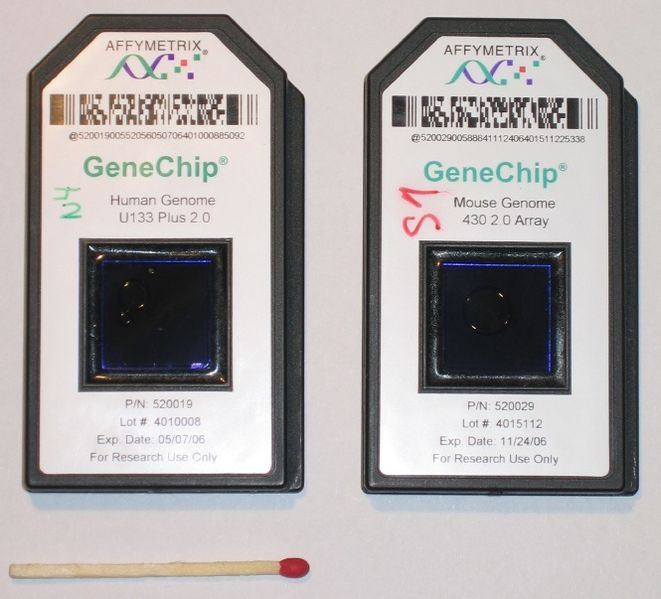
\includegraphics[width=0.9\textwidth]{Affymetrix-microarray}
      \end{figure}
    \end{column}
    \begin{column}{0.5\textwidth}
      \begin{figure}
        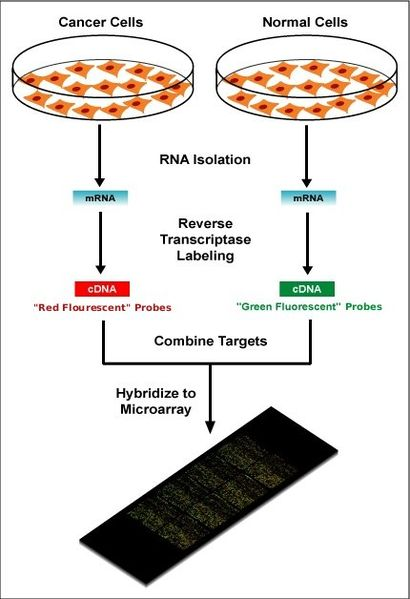
\includegraphics[width=0.9\textwidth]{Microarray-schema}
      \end{figure}
    \end{column}
  \end{columns}
  \source{en.wikipedia.org}
  \note{http://en.wikipedia.org/wiki/DNA_microarray}
\end{frame}

\begin{frame}[plain]
  \frametitle{Van't Veer breast-cancer data}
\begin{figure}
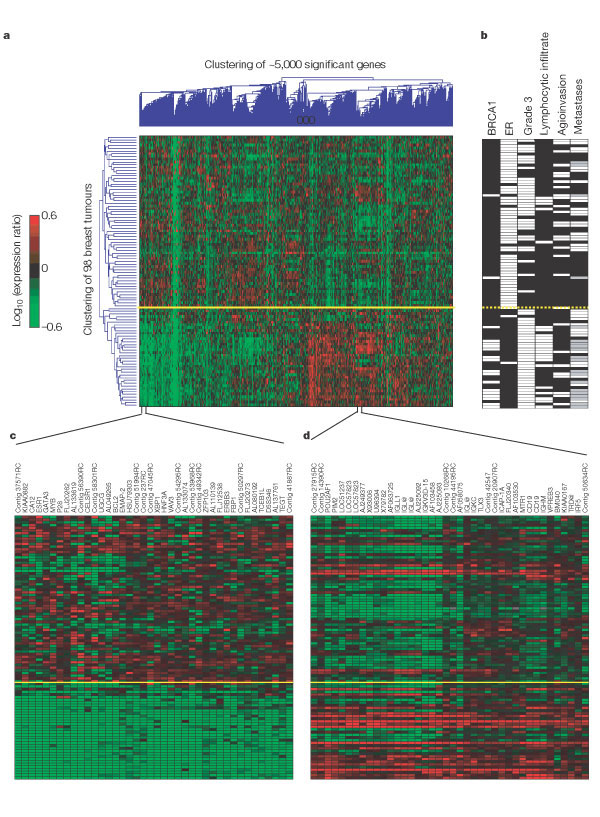
\includegraphics[height=1\textheight]{vantveer-summary}
\end{figure}
\source{Laura J. van 't Veer et.al. Nature, (2002)}
\note{a, Two-dimensional presentation of transcript ratios for 98 breast tumours. There were 4,968 significant genes across the group. Each row represents a tumour and each column a single gene. As shown in the colour bar, red indicates upregulation, green downregulation, black no change, and grey no data available. The yellow line marks the subdivision into two dominant tumour clusters. b, Selected clinical data for the 98 patients in a: BRCA1 germline mutation carrier (or sporadic patient), ER expression, tumour grade 3 (versus grade 1 and 2), lymphocytic infiltrate, angioinvasion, and metastasis status. White indicates positive, black negative and grey denotes tumours derived from BRCA1 germline carriers who were excluded from the metastasis evaluation. The cluster below the yellow line consists of 36 tumours, of which 34 are ER negative (total 39 ER-negative) and 16 are carriers of the BRCA1 mutation (total 18). c, Enlarged portion from a containing a group of genes that co-regulate with the ER- gene (ESR1). Each gene is labelled by its gene name or accession number from GenBank. Contig ESTs ending with RC are reverse-complementary of the named contig EST. d, Enlarged portion from a containing a group of co-regulated genes that are the molecular reflection of extensive lymphocytic infiltrate, and comprise a set of genes expressed in T and B cells. (Gene annotation as in c.)}
\note{http://www.nature.com/nature/journal/v415/n6871/full/415530a.html}
\end{frame}

\begin{frame}[plain]
  \frametitle{Yeast Protein Interaction Network}
\begin{figure}
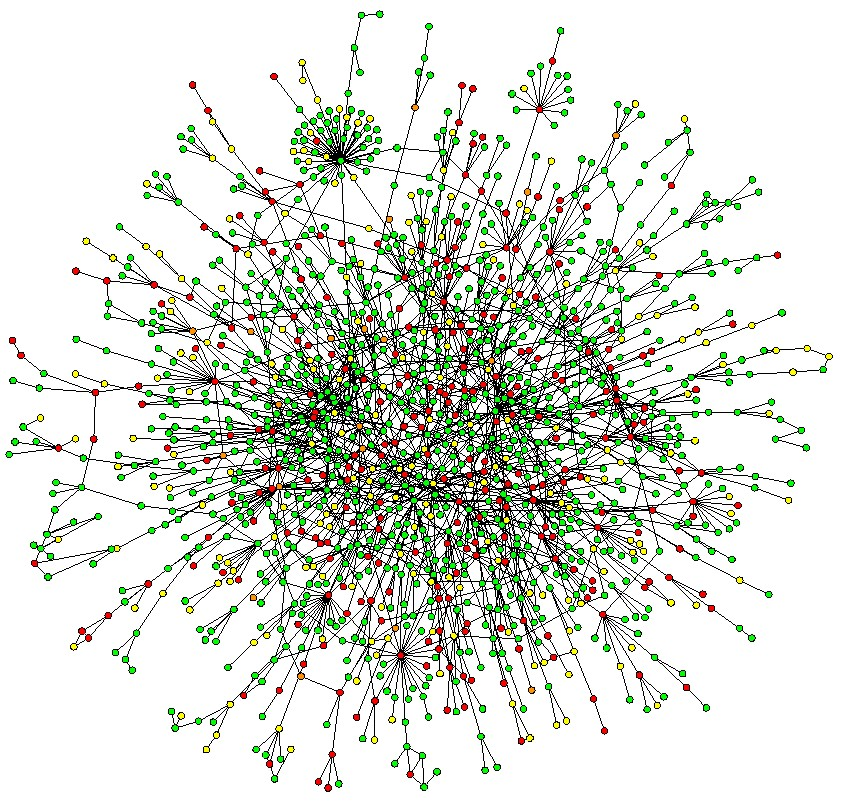
\includegraphics[width=0.8\textwidth]{yeastProteinInteractionNetwork}
\end{figure}
\note{http://www.bordalierinstitute.com/images/yeastProteinInteractionNetwork.jpg}
\source{http://osf1.gmu.edu/~rcouch/chem665.htm}
\end{frame}


\section{Formulation} 

\begin{frame}
\begin{figure}
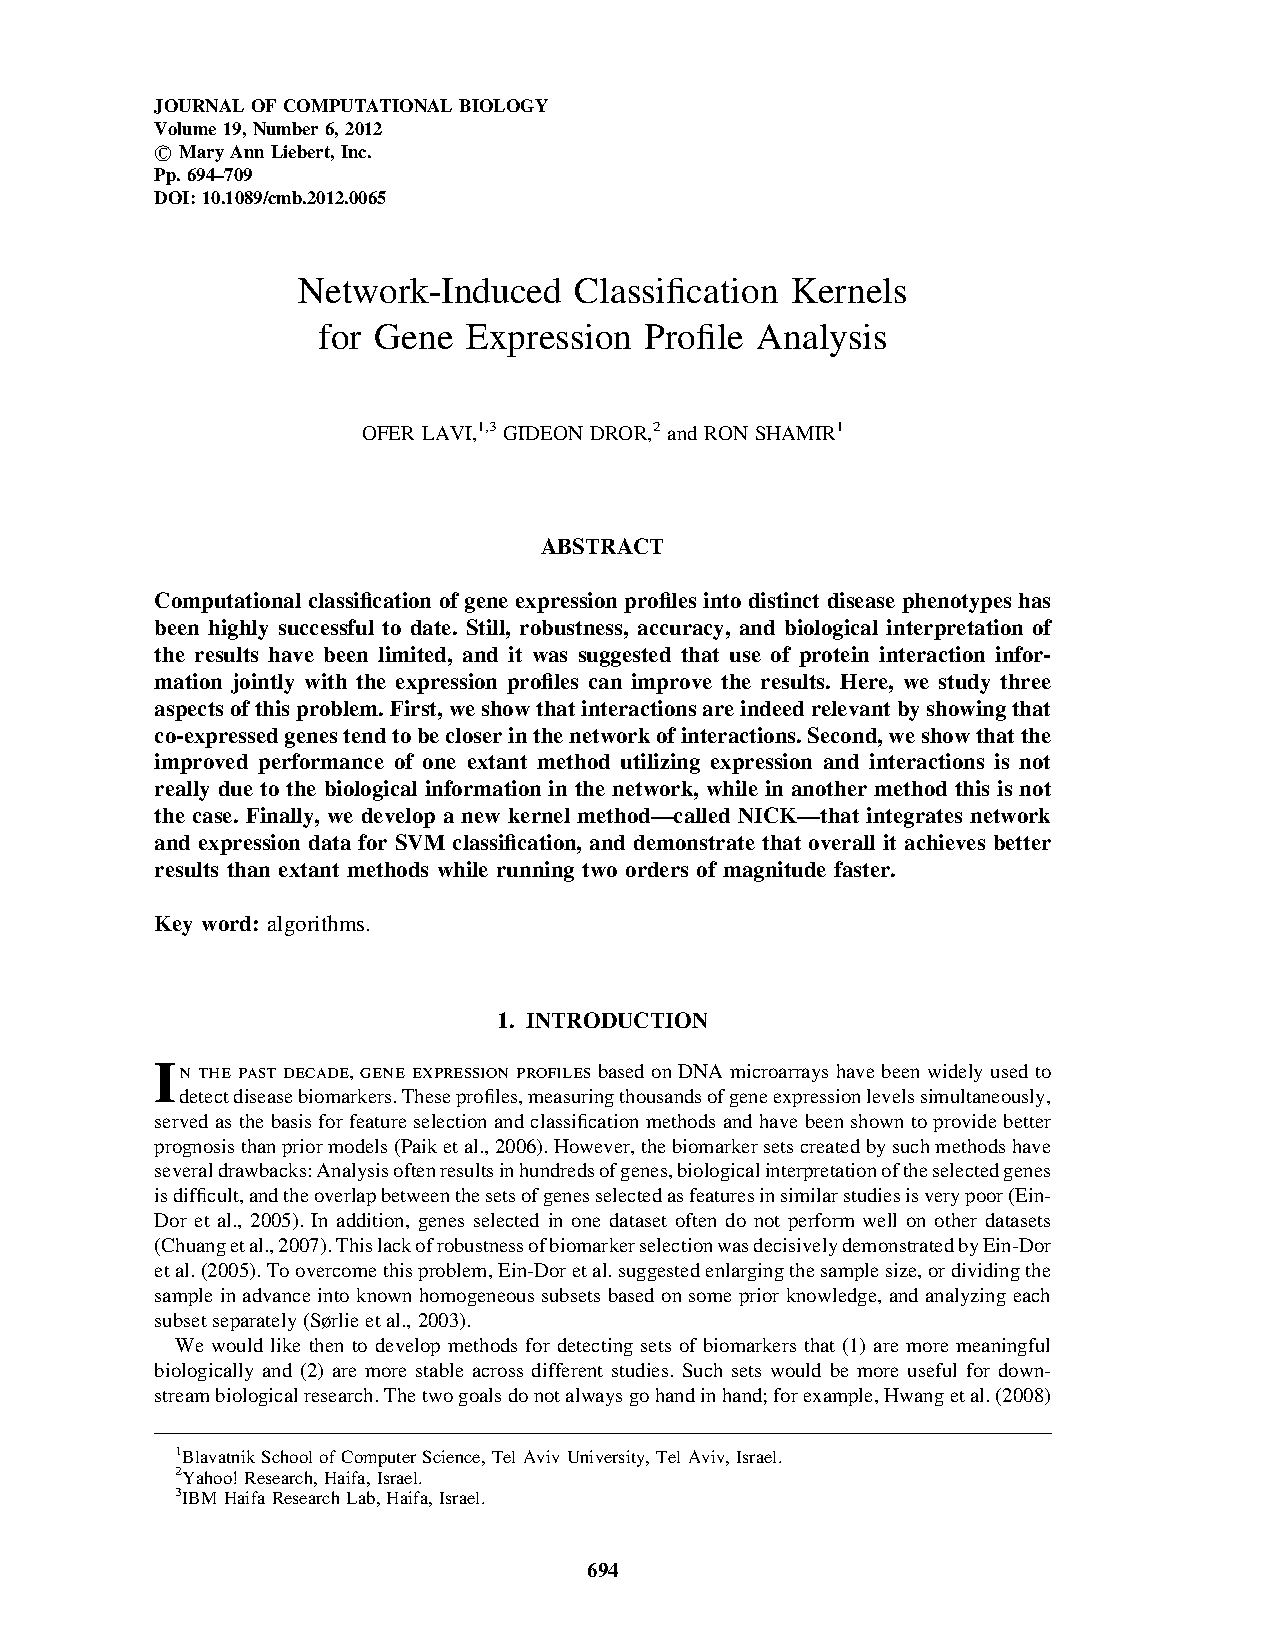
\includegraphics[height=1\textheight]{NICK-page1}
\end{figure}
\end{frame}


\begin{frame}
  \frametitle{NICK}
  \begin{columns}
    \begin{column}{0.5\textwidth}
      
      \begin{block}{\tiny{1. SVM modified objective function}}
        \tiny
        \begin{center}
          $\min_{\mathbf{w}, w_0}\left\{\frac{1}{2}\|\mathbf{w}\|^2 + \frac{1}{2}\beta\sum_{(j,k)\in E}(w_j-w_k)^2\right\}$
        \end{center}
        s.t.:
        \begin{center}
          $\forall i \in \{1,\cdots,n\} : (\mathbf{w}\mathbf{x}_i+w_0)y_i\geq 1$
        \end{center}
      \end{block}
      
      \begin{block}{\tiny{3. Dual to Primal}}
        \tiny
        \begin{center}
          $\mathbf{w} = (\mathbf{I} + \beta \mathbf{B})^{-1} \sum_{i = 1}^n \alpha_i y_i \mathbf{x}_i$
        \end{center}
      \end{block}
    \end{column}
    
    \begin{column}{0.5\textwidth}
      \begin{block}{\tiny{2. Dual problem}}
        \tiny
        \begin{center}
          \begin{align*}
            &\max_\alpha\left\{\sum_{i=1}^n\alpha_i-\frac{1}{2}\sum_{i=1}^n\sum_{j=1}^n\alpha_i\alpha_j y_i y_j (\mathbf{x}_i^T\mathbf{L})(\mathbf{L}^T\mathbf{x}_j)\right\}\\
            &\mathbf{L}\mathbf{L}^T=(\mathbf{I}+\beta \mathbf{B})^{-1}\\
            \text{s.t.: }&\\
            &\forall i \in \{1,\cdots,n\}: \sum_{i=1}^n\alpha_iy_i=0\\
            &\forall i \in \{1,\cdots,n\}: \alpha_i \geq 0
          \end{align*}
        \end{center}
      \end{block}
    \end{column}
  \end{columns}
  \source{Ofer Lavi, et.al., Journal of Computational Biology, (2012)}
\end{frame}

\begin{frame}
  \frametitle{NICK Performance Summary}
  \begin{figure}
    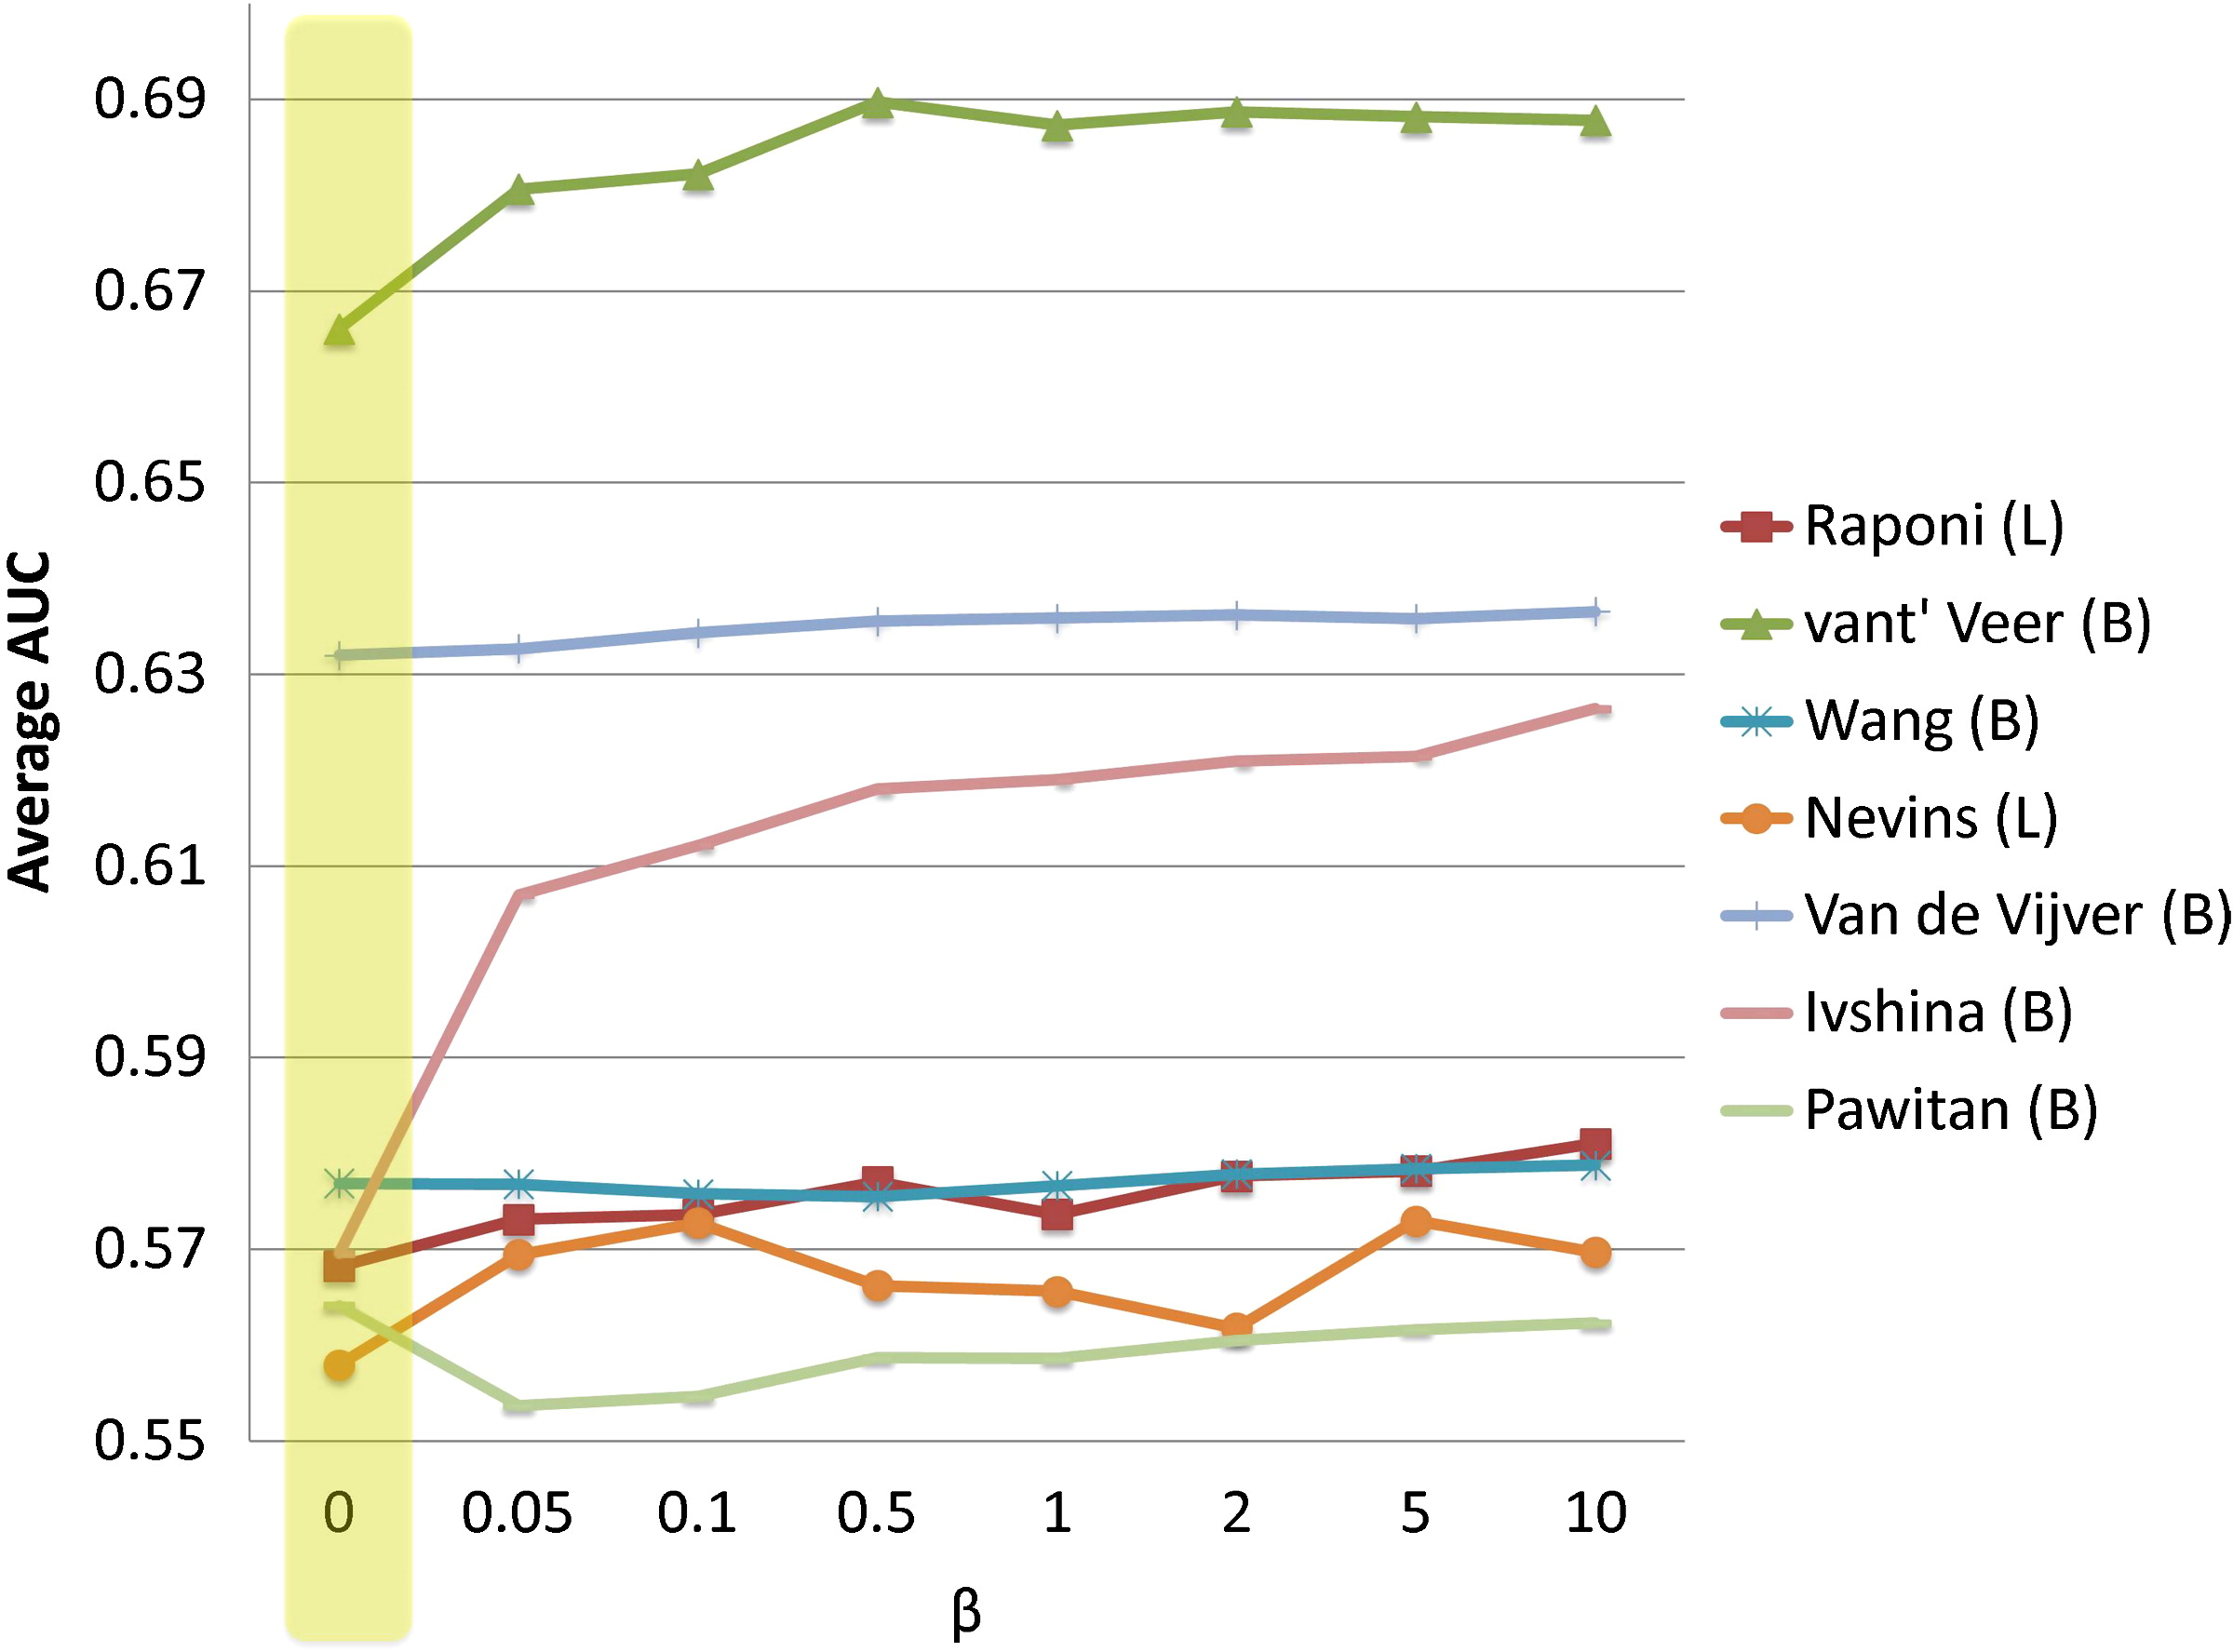
\includegraphics[width=0.8\textwidth]{NICK-perfs}
  \end{figure}
  \source{Ofer Lavi, et.al., Journal of Computational Biology, (2012)}
  \note{http://online.liebertpub.com/doi/full/10.1089/cmb.2012.0065}
\end{frame}


\section{Results}
\begin{frame}
\frametitle{Synthesize data}
\begin{enumerate}
\item A random graph
\item Signal nodes: \[ f(n) = \left\{ 
  \begin{array}{l l}
    N(-\mu, 1) & \quad \text{if $n$ is in class $1$}\\
    N(\mu, 1) & \quad \text{if $n$ is in class $2$}
  \end{array} \right.\]
\item Random nodes: \[f(n) = N(0, 1) \]
\item Pathway: 2, 3, or 4 connected signal nodes.
\end{enumerate}
\end{frame}

\begin{frame}[plain]
  \frametitle{Synthesized data}
  \begin{figure}
    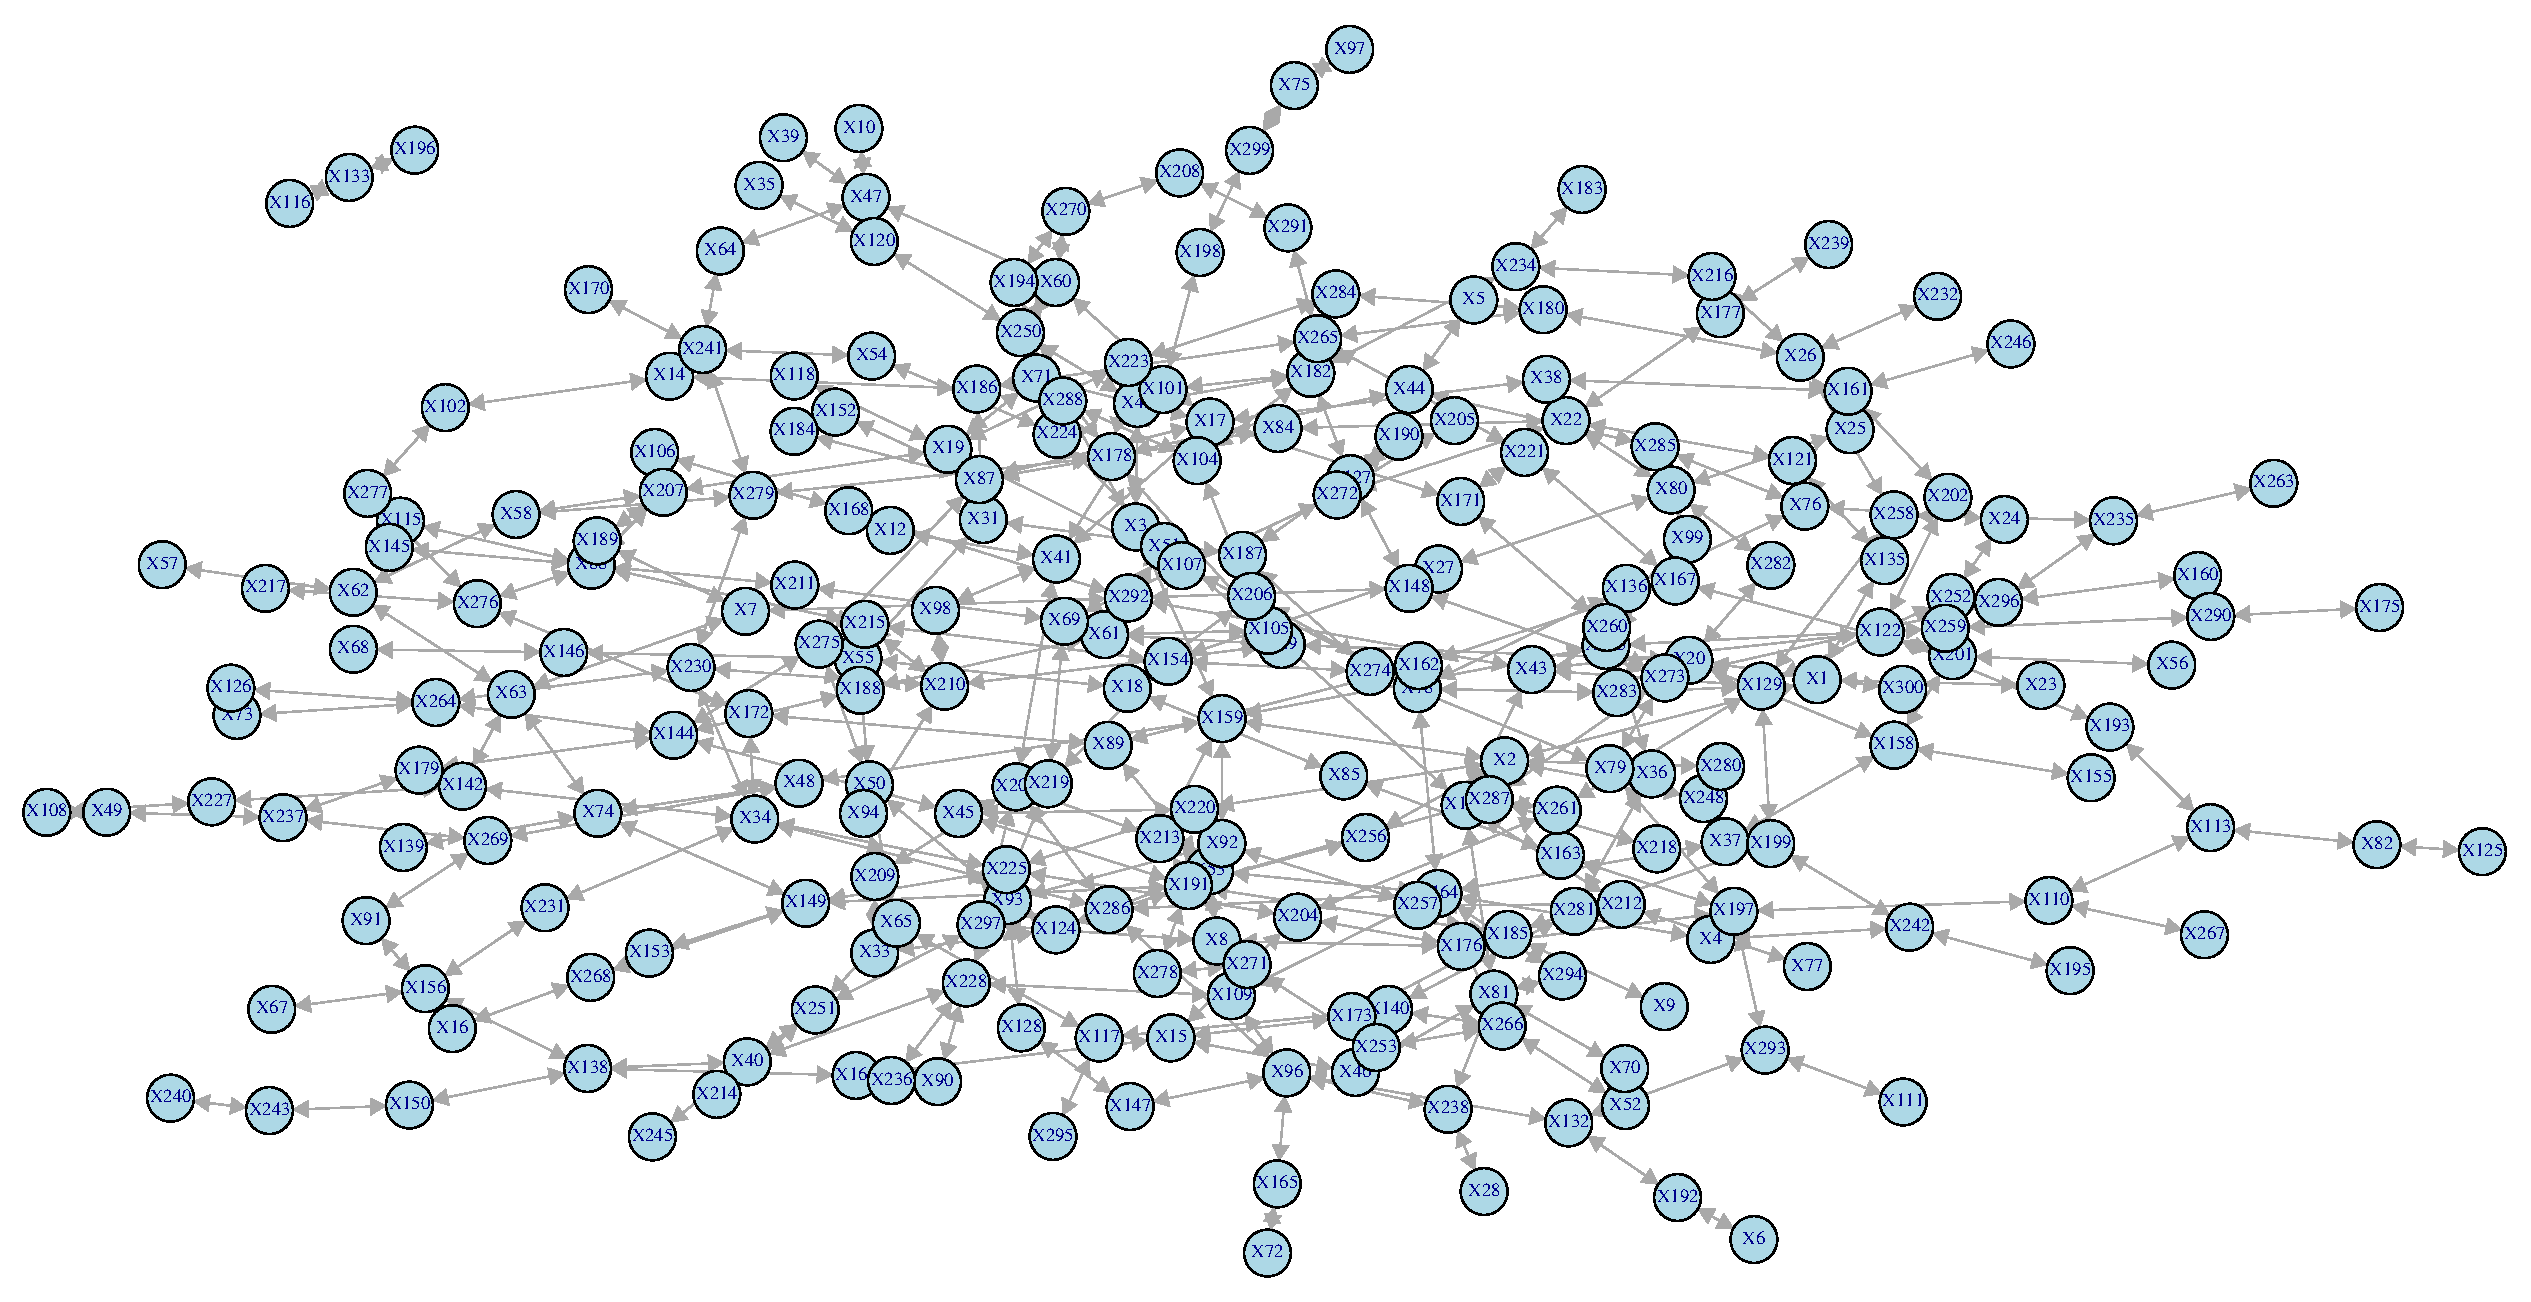
\includegraphics[width=0.8\textwidth]{synthesized}
  \end{figure}
\end{frame}

\begin{frame}[plain]
  \frametitle{Synthesized data easy scenario}
  \begin{figure}
    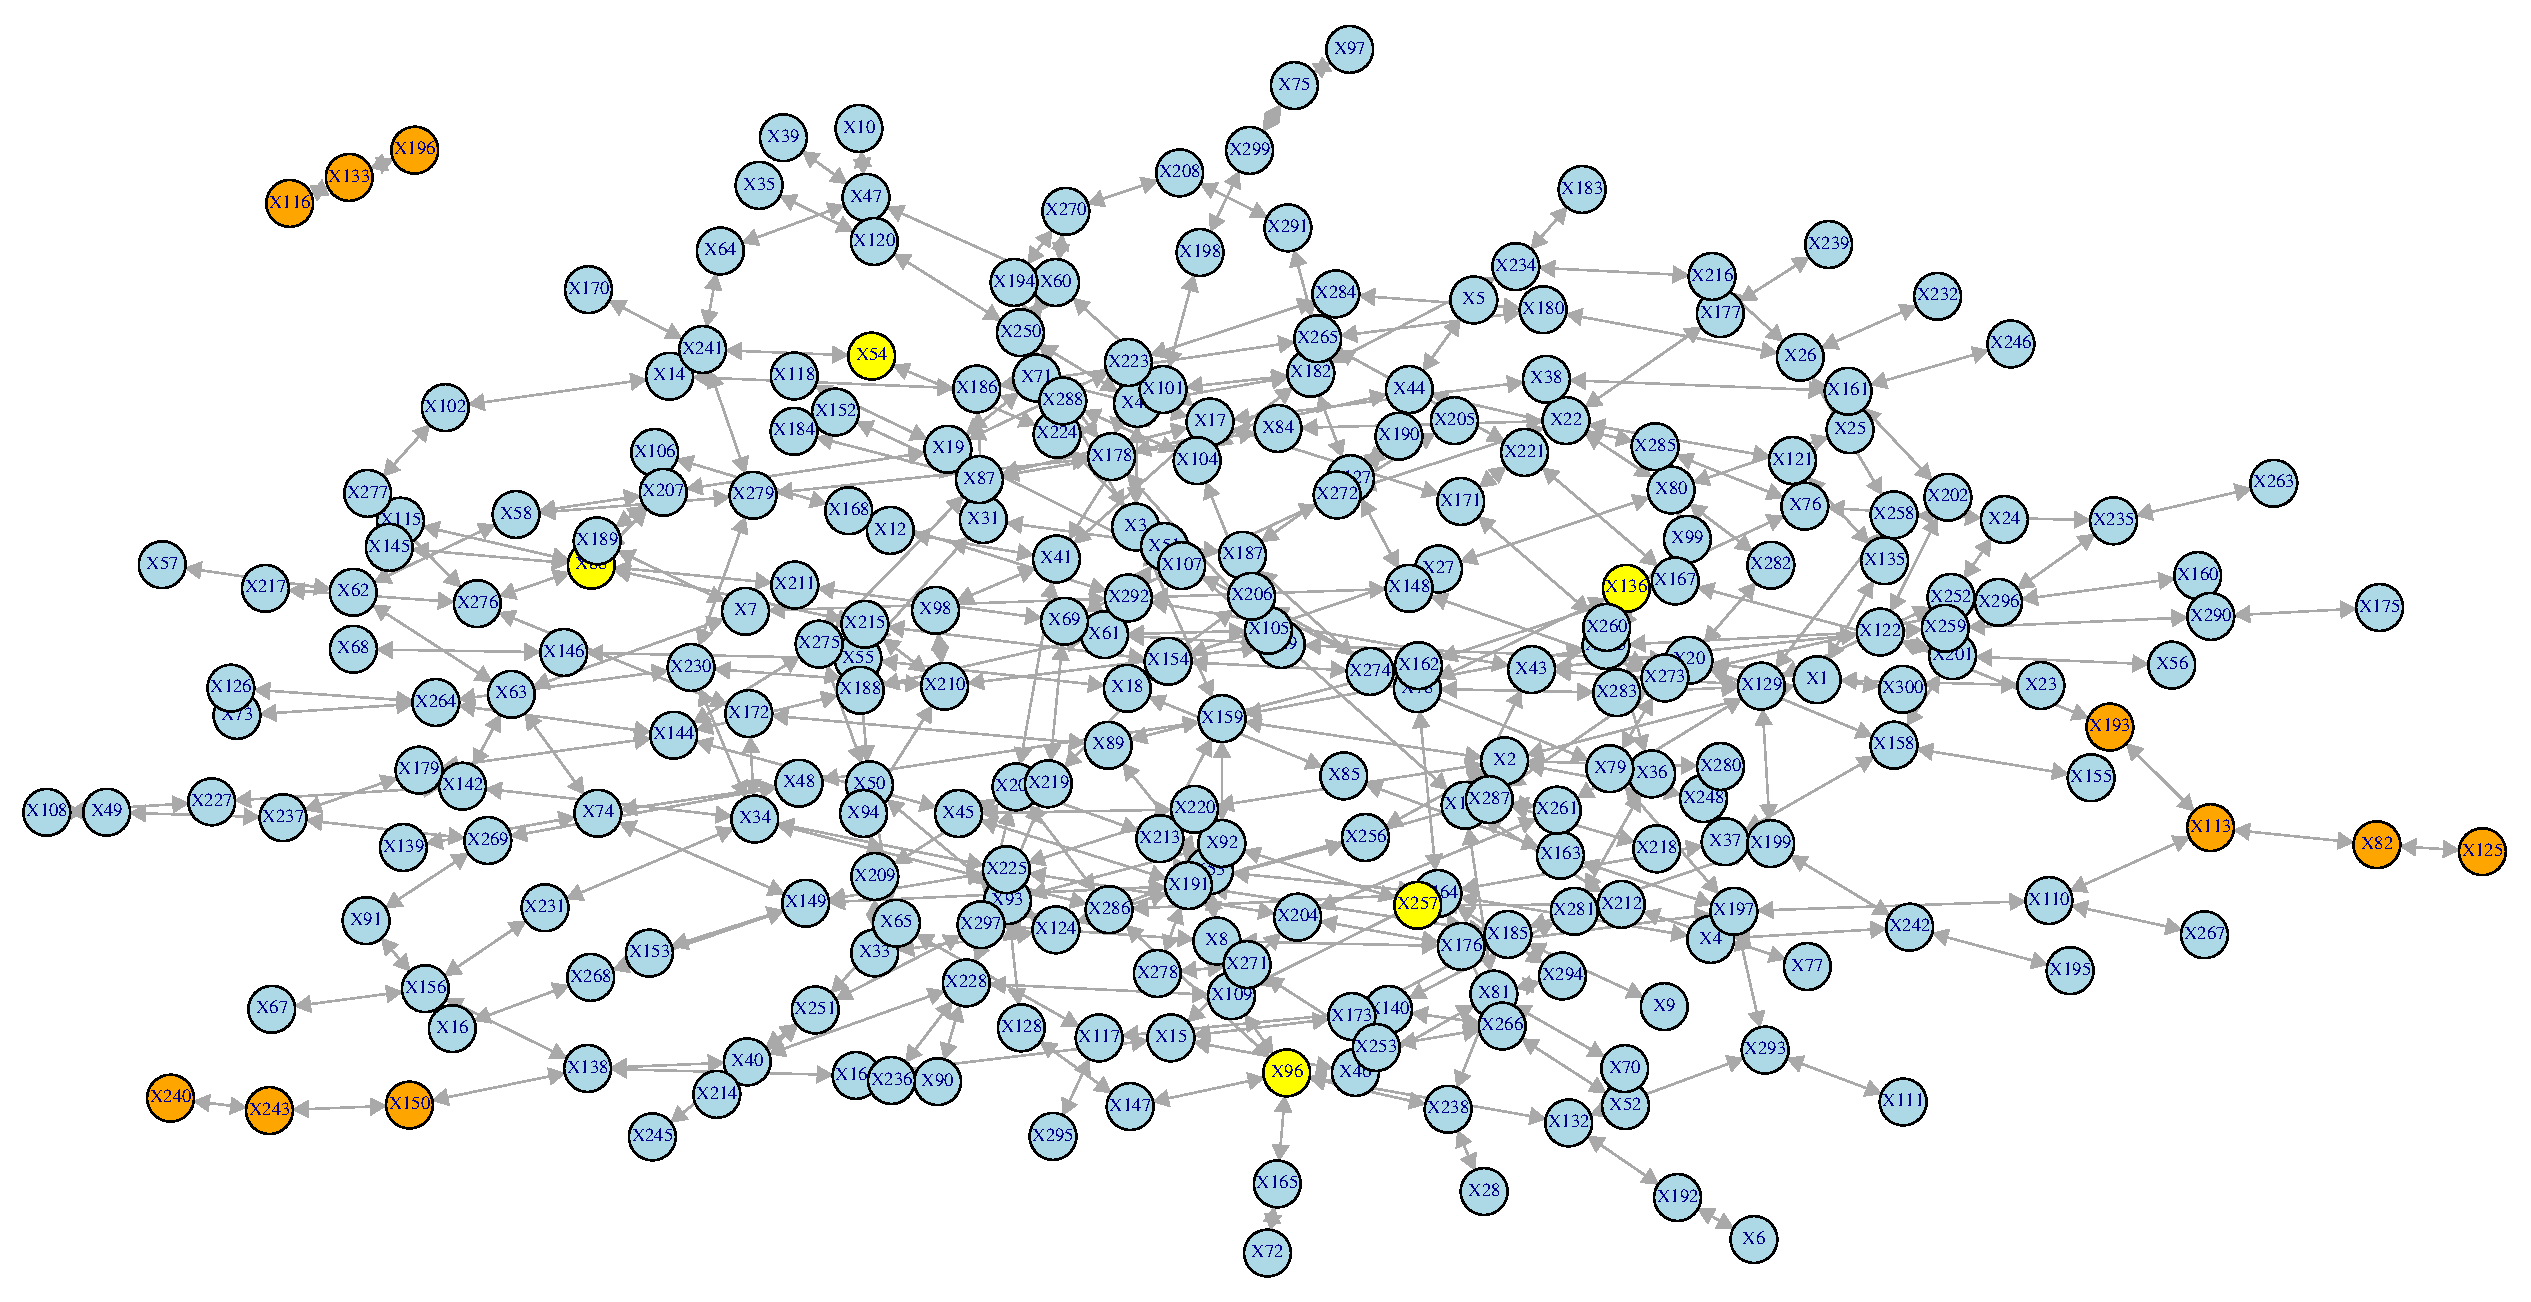
\includegraphics[width=0.8\textwidth]{synthesized-easy}
  \end{figure}
\end{frame}
\begin{frame}[plain]
  \frametitle{Synthesized data easy scenario}
  \begin{figure}
    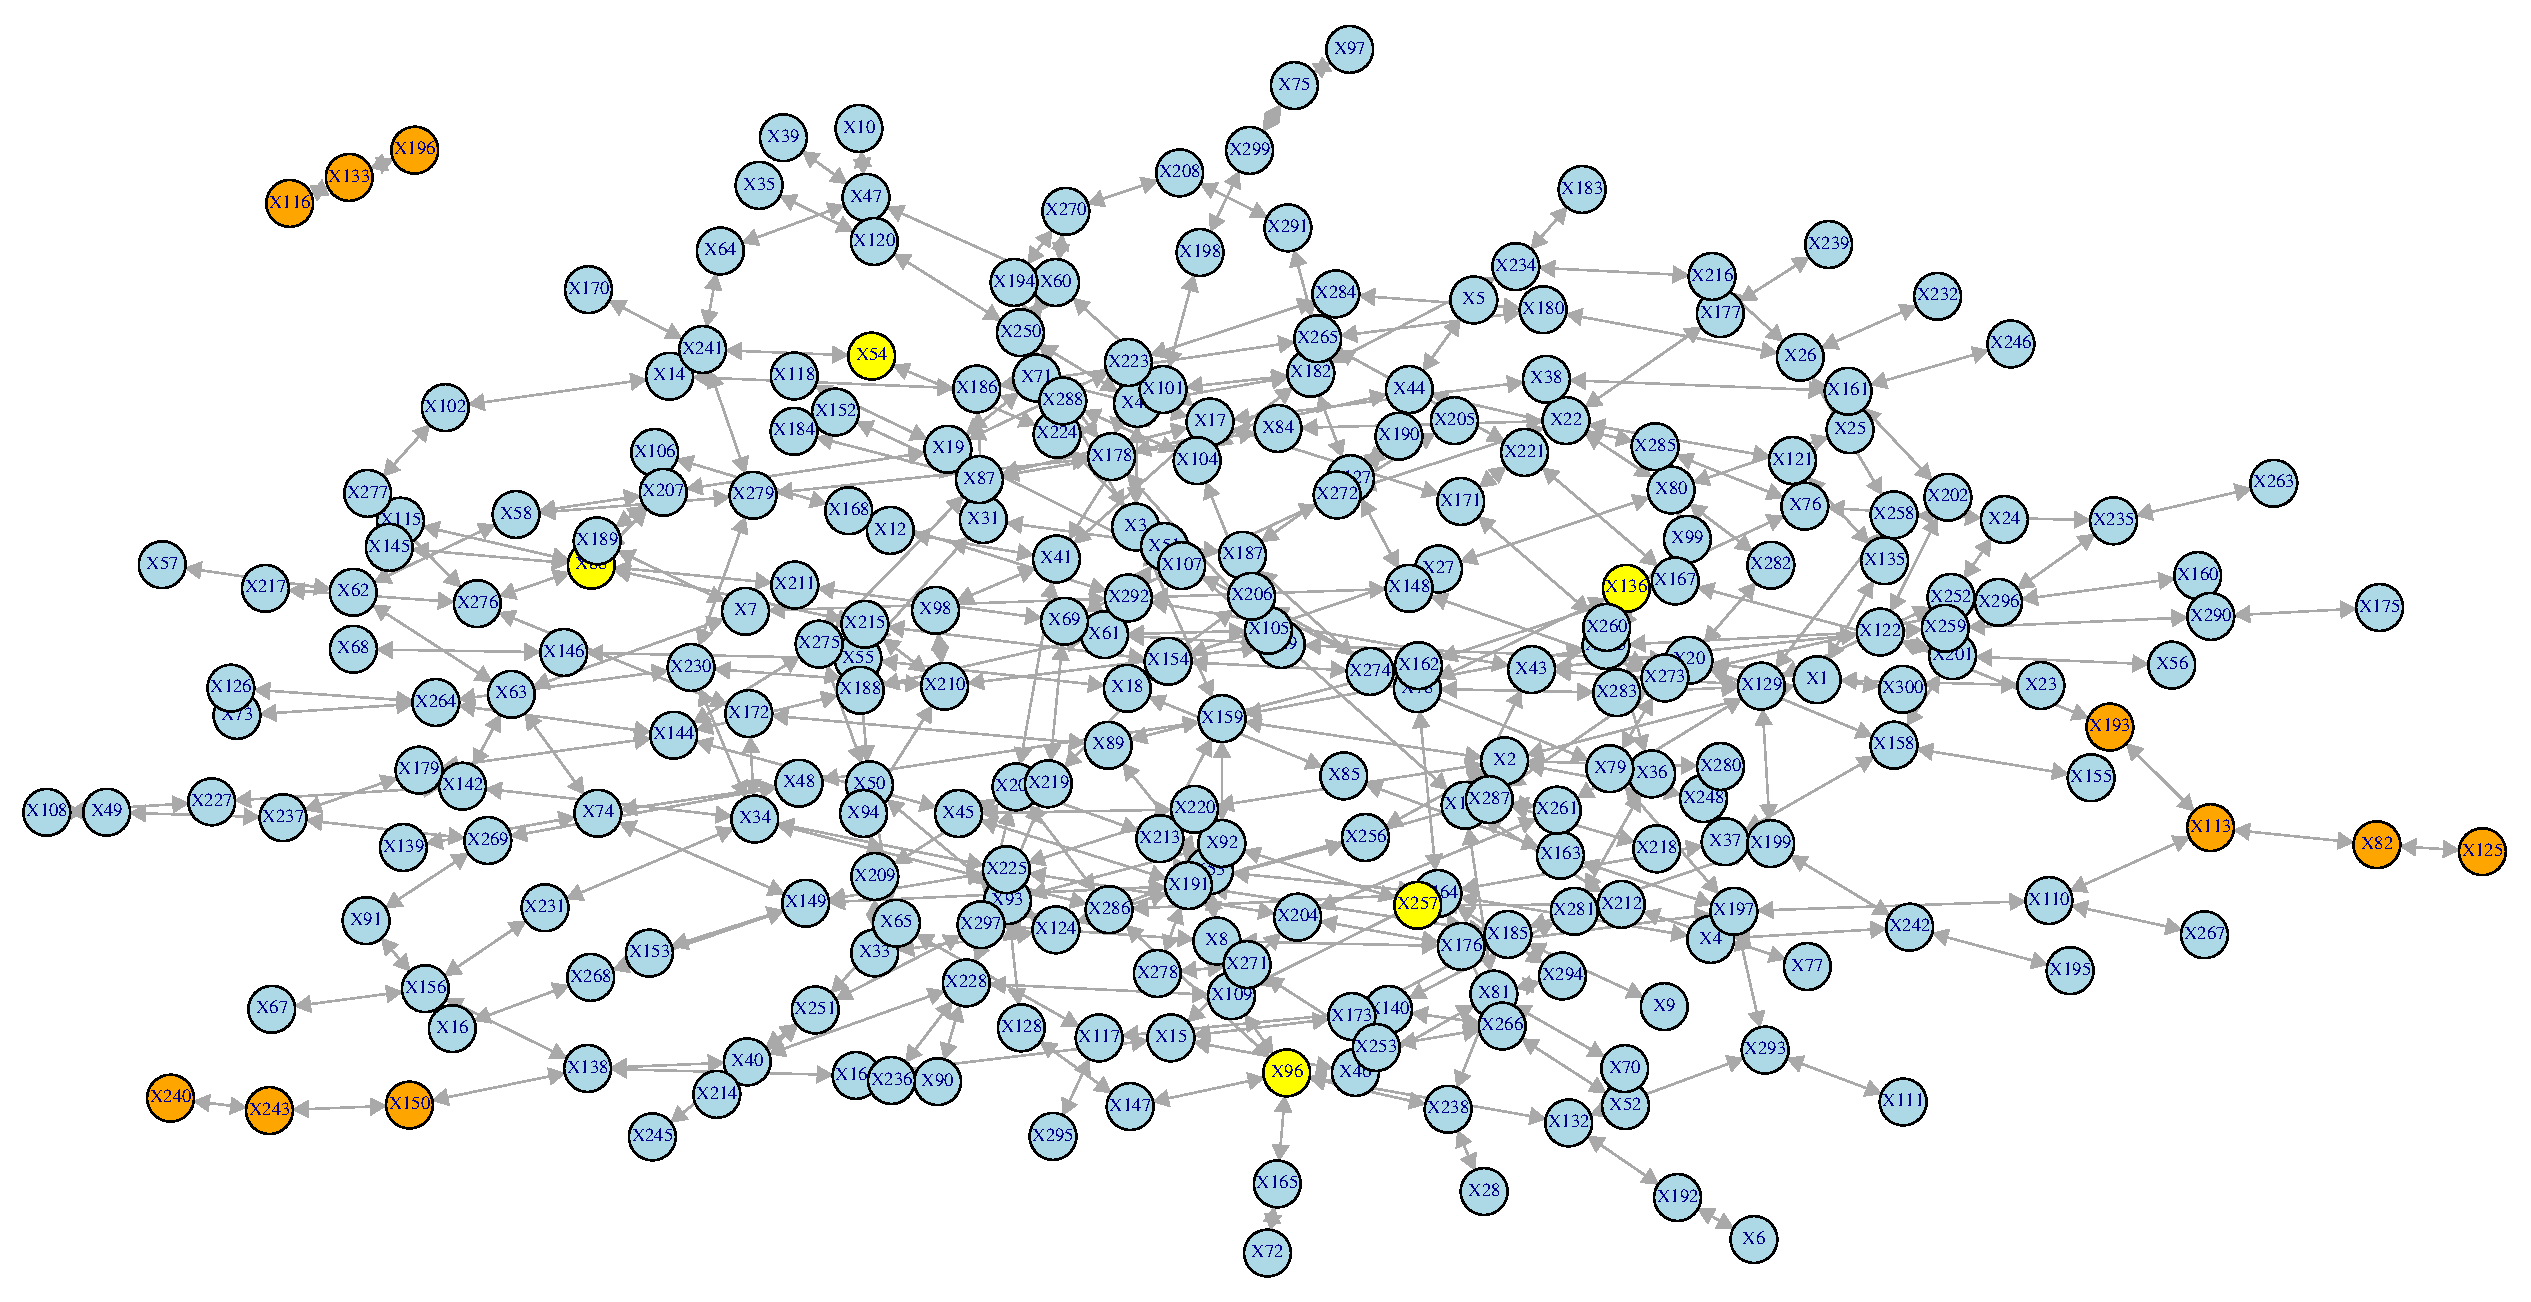
\includegraphics[width=0.8\textwidth]{synthesized-easy}
  \end{figure}
  \begin{textblock*}{\paperwidth}(0.01\textwidth,0.2\textheight)
    \raggedright 
    \tiny
    \begin{tabular}{| c c |}
      \hline
\boz X116   &  \boz X116  \\ \hline
\boz X125   &  \boz X125  \\ \hline
\boz X116   &  \boz X133  \\ \hline
\boz X125   &  \boz X82  \\ \hline
\boz X240   &  \boz X240  \\ \hline
\boz X196   &  \boz X196  \\ \hline
\boz X196   &  \boz X133  \\ \hline
\boz X133   &  \boz X133  \\ \hline
\boz X82   &  \boz X82  \\ \hline
\boz X240   &  \boz X243  \\ \hline
\boz X82   &  \boz X113  \\ \hline
X6   &  X6  \\ \hline
\ghool X257   &  \ghool X257  \\ \hline
X6   &  X192  \\ \hline
\ghool X257   &  X212  \\ \hline
\boz X243   &  \boz X243  \\ \hline
X212   &  X212  \\ \hline
X192   &  X192  \\ \hline
\ghool X257   &  X92  \\ \hline
X72   &  X72  \\ \hline
X172   &  X172  \\ \hline
X72   &  X165  \\ \hline
X212   &  X77  \\ \hline
X57   &  X57  \\ \hline
X165   &  X165  \\ \hline
X192   &  X132  \\ \hline
X92   &  X92  \\ \hline
X118   &  X118  \\ \hline
\boz X243   &  \boz X150  \\ \hline
X77   &  X77  \\ \hline
    \end{tabular}
    \hspace{.5em}
  \end{textblock*}
  \begin{textblock*}{\paperwidth}(1\textwidth,0.2\textheight)
    \raggedright 
    \tiny
    \begin{tabular}{| c c |}
      \hline
\boz X196   &  \boz X196  \\ \hline
\boz X196   &  \boz X133  \\ \hline
\boz X133   &  \boz X133  \\ \hline
\boz X133   &  \boz X116  \\ \hline
\boz X116   &  \boz X116  \\ \hline
\boz X240   &  \boz X240  \\ \hline
\boz X125   &  \boz X125  \\ \hline
\boz X240   &  \boz X243  \\ \hline
\boz X125   &  \boz X82  \\ \hline
\boz X243   &  \boz X243  \\ \hline
\boz X196   &  \boz X116  \\ \hline
\boz X82   &  \boz X82  \\ \hline
\boz X243   &  \boz X150  \\ \hline
\boz X82   &  \boz X113  \\ \hline
\boz X150   &  \boz X150  \\ \hline
X157   &  X157  \\ \hline
X6   &  X6  \\ \hline
\boz X113   &  \boz X113  \\ \hline
X6   &  X192  \\ \hline
X95   &  X95  \\ \hline
X192   &  X192  \\ \hline
\boz X113   &  X110  \\ \hline
X72   &  X72  \\ \hline
X267   &  X267  \\ \hline
X249   &  X249  \\ \hline
X72   &  X165  \\ \hline
X192   &  X132  \\ \hline
X267   &  X110  \\ \hline
\boz X150   &  X138  \\ \hline
X110   &  X110  \\ \hline
    \end{tabular}
    \hspace{.5em}
  \end{textblock*}
\end{frame}

\begin{frame}[plain]
  \frametitle{Synthesized data medium scenario}
  \begin{figure}
    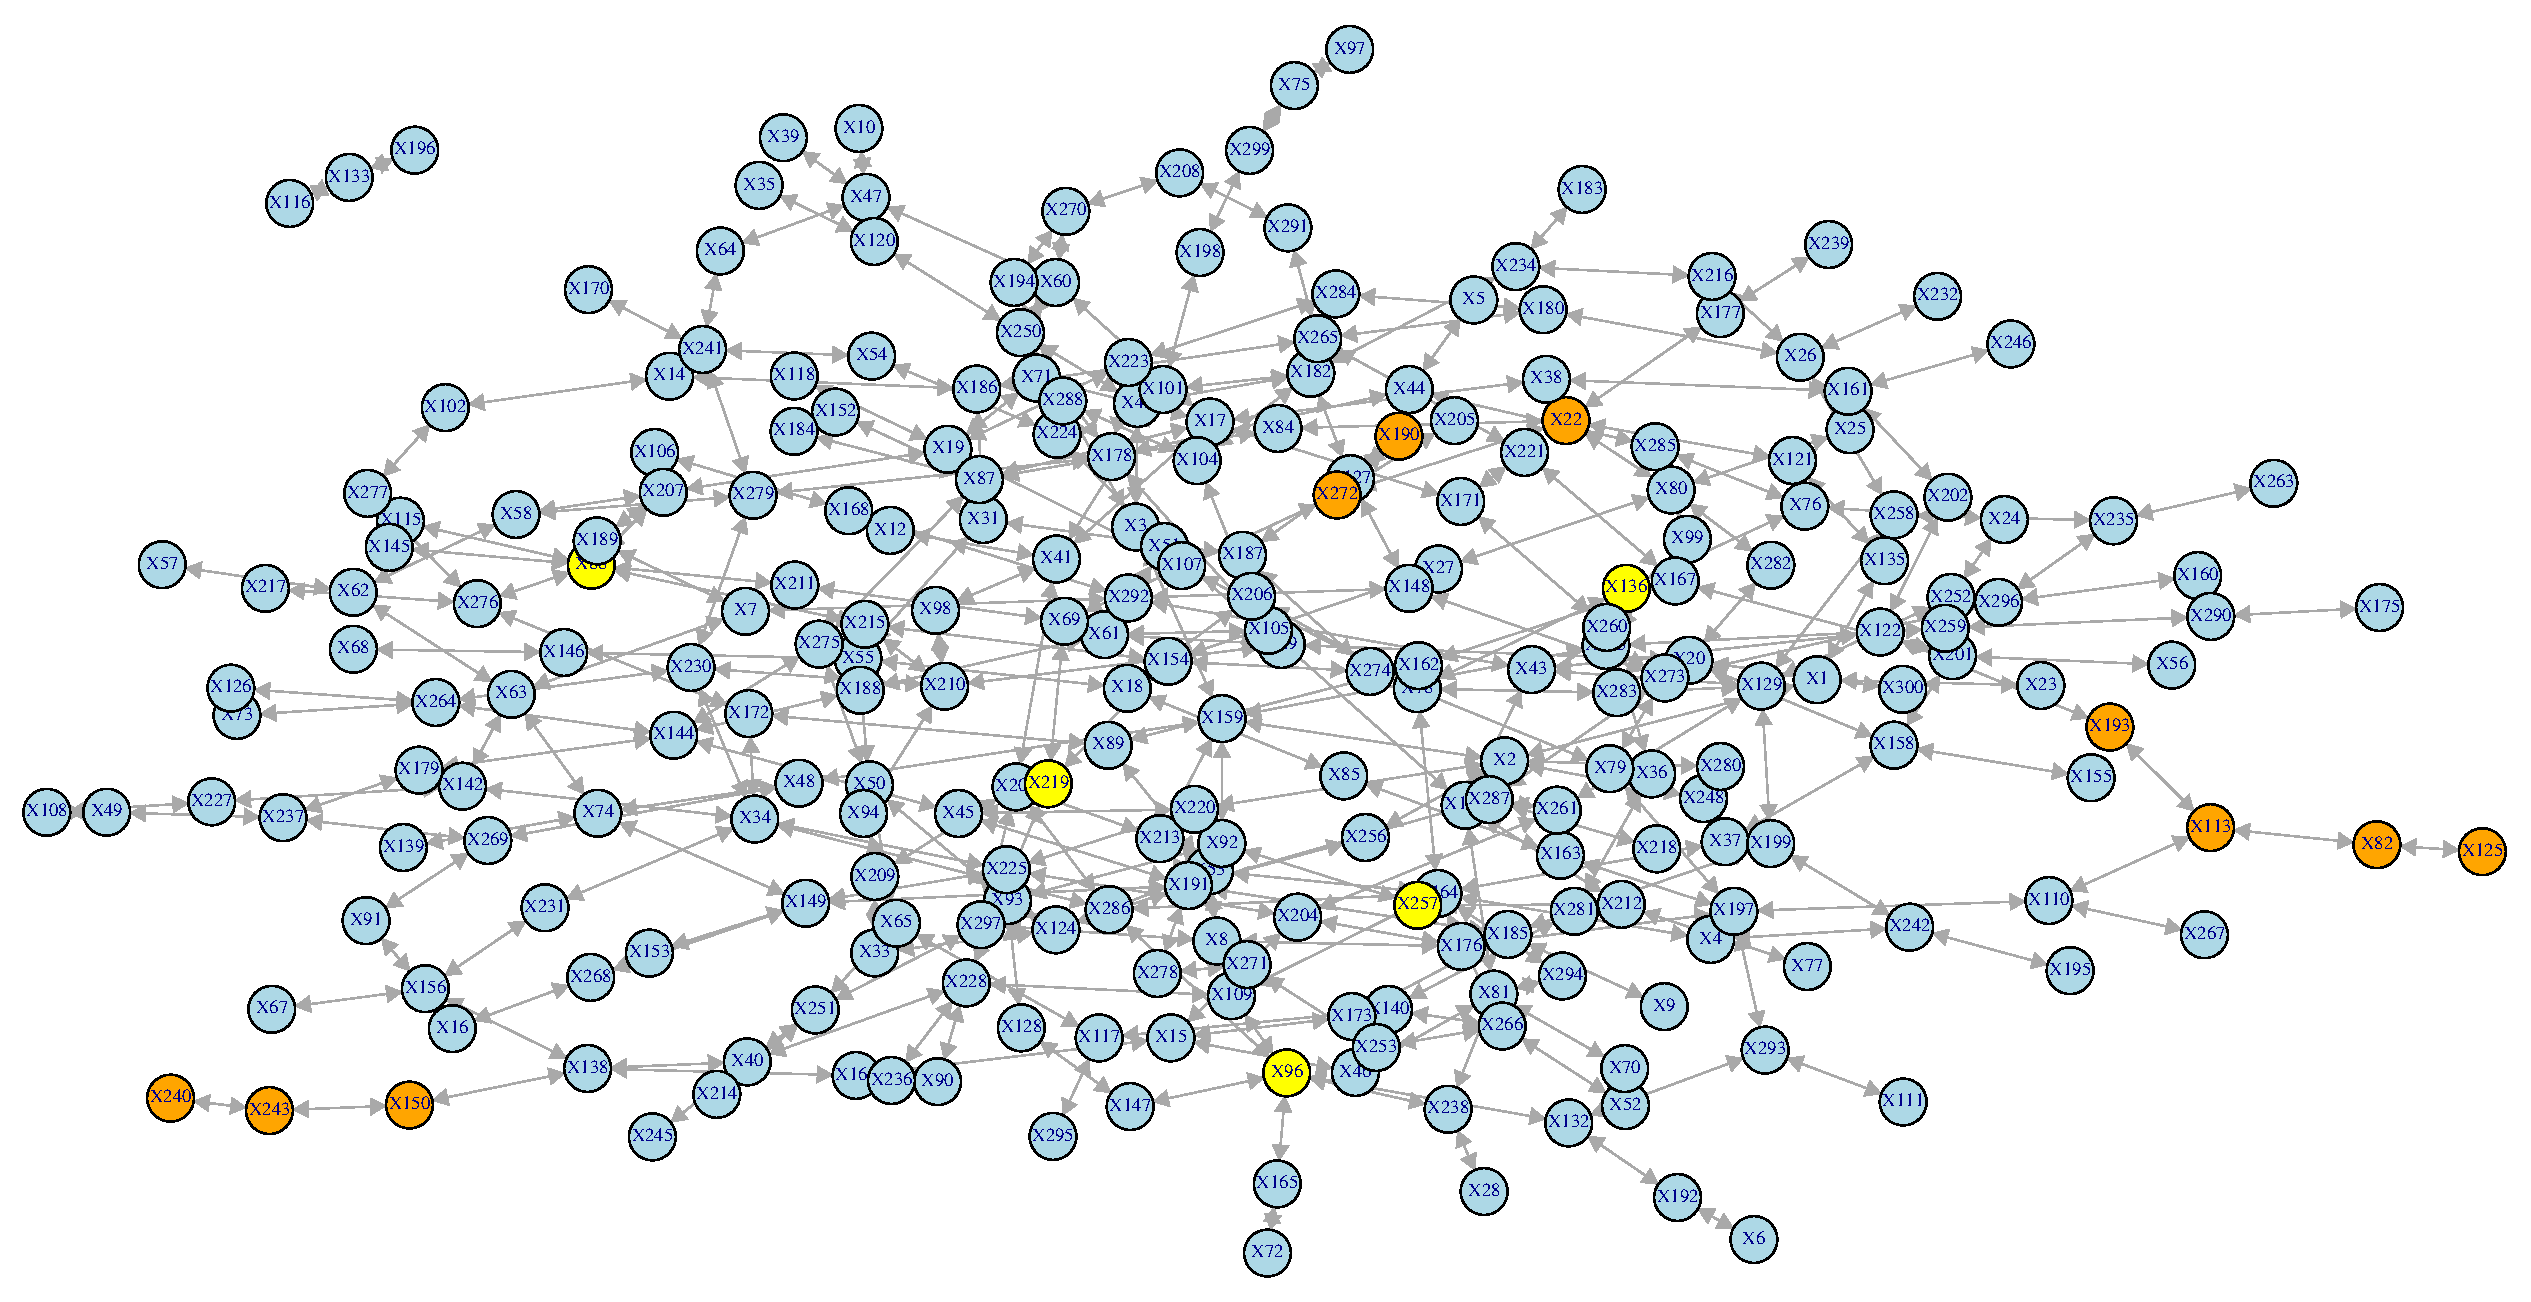
\includegraphics[width=0.8\textwidth]{synthesized-medium}
  \end{figure}
\end{frame}
\begin{frame}[plain]
  \frametitle{Synthesized data medium scenario}
  \begin{figure}
    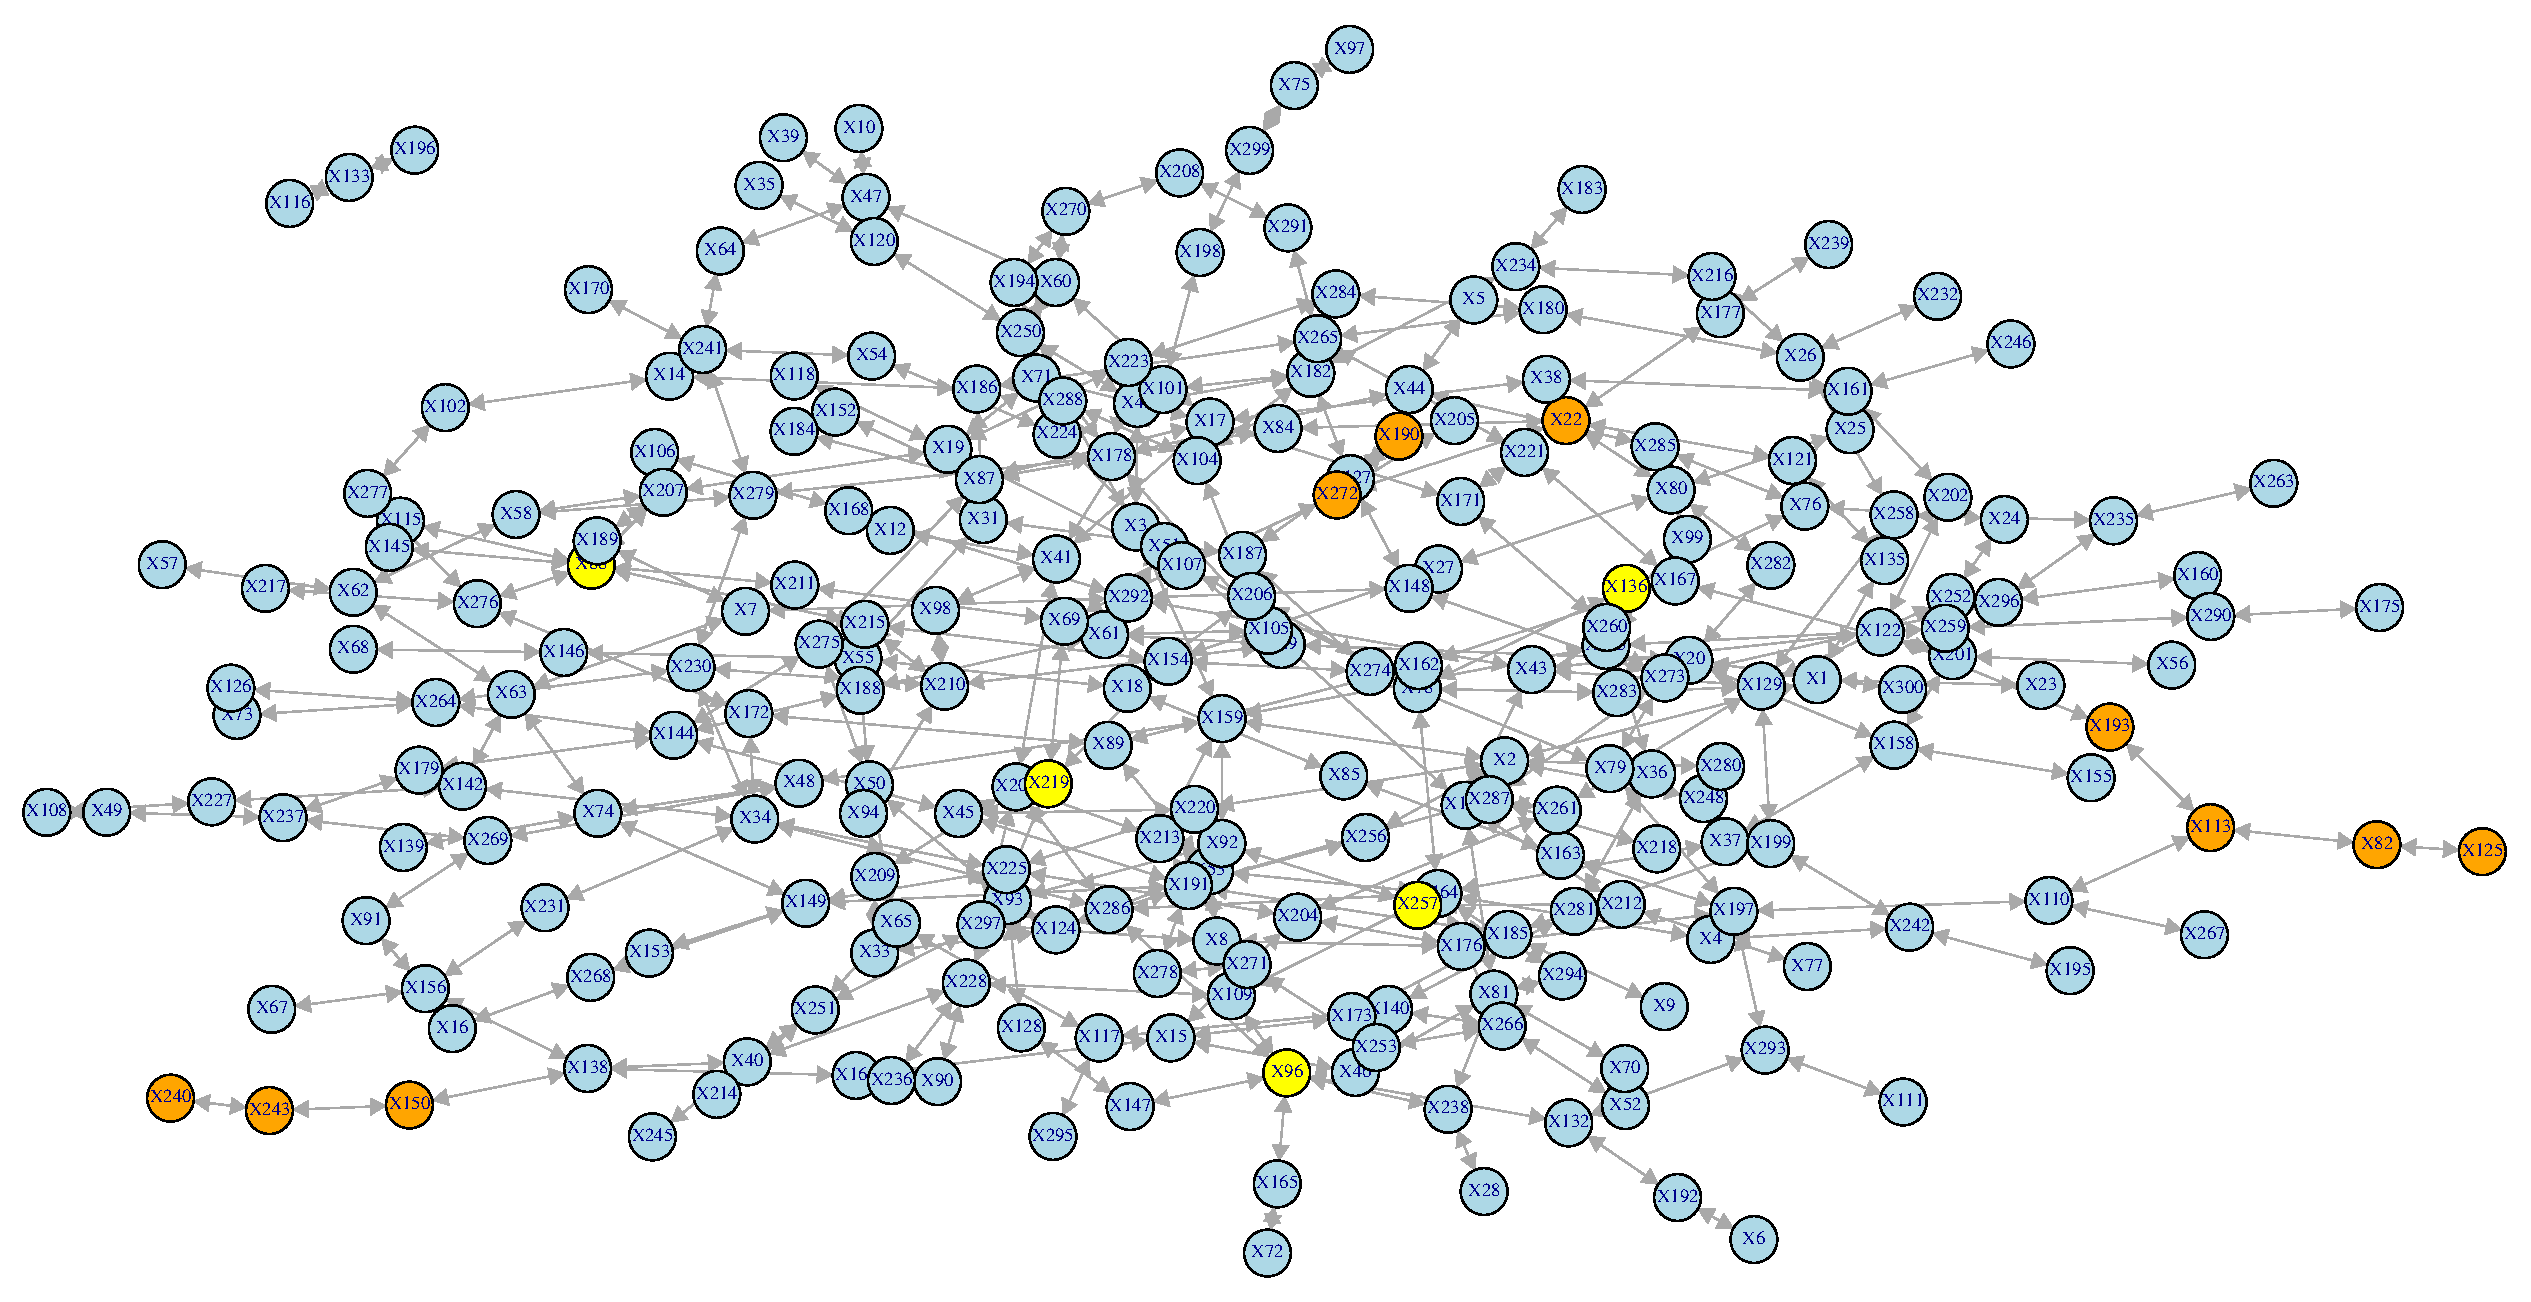
\includegraphics[width=0.8\textwidth]{synthesized-medium}
  \end{figure}
  \begin{textblock*}{\paperwidth}(0.01\textwidth,0.2\textheight)
    \raggedright 
    \tiny
    \begin{tabular}{| c c |}
      \hline
\boz X125   &  \boz X125  \\ \hline
\boz X125   &  \boz X82  \\ \hline
X267   &  X267  \\ \hline
X69   &  X69  \\ \hline
X69   &  \ghool X219  \\ \hline
X267   &  X110  \\ \hline
\boz X240   &  \boz X240  \\ \hline
X69   &  \boz X272  \\ \hline
\ghool X219   &  \ghool X219  \\ \hline
\boz X82   &  \boz X82  \\ \hline
\ghool X219   &  X154  \\ \hline
\boz X82   &  \boz X113  \\ \hline
X154   &  X154  \\ \hline
X110   &  X110  \\ \hline
\boz X240   &  \boz X243  \\ \hline
X110   &  \boz X113  \\ \hline
\boz X113   &  \boz X113  \\ \hline
\boz X272   &  \boz X272  \\ \hline
\boz X272   &  X205  \\ \hline
X205   &  X205  \\ \hline
\boz X243   &  \boz X243  \\ \hline
X10   &  X10  \\ \hline
X176   &  X176  \\ \hline
X154   &  X274  \\ \hline
X77   &  X77  \\ \hline
X33   &  X33  \\ \hline
X85   &  X85  \\ \hline
X110   &  X197  \\ \hline
X69   &  X211  \\ \hline
X154   &  X27  \\ \hline
    \end{tabular}
    \hspace{.5em}
  \end{textblock*}
  \begin{textblock*}{\paperwidth}(1\textwidth,0.2\textheight)
    \raggedright 
    \tiny
    \begin{tabular}{| c c |}
      \hline
\boz X125   &  \boz X125  \\ \hline
\boz X125   &  \boz X82  \\ \hline
\boz X240   &  \boz X240  \\ \hline
\boz X82   &  \boz X82  \\ \hline
\boz X240   &  \boz X243  \\ \hline
X267   &  X267  \\ \hline
\boz X82   &  \boz X113  \\ \hline
\boz X243   &  \boz X243  \\ \hline
X267   &  X110  \\ \hline
\boz X113   &  \boz X113  \\ \hline
\boz X113   &  X110  \\ \hline
X110   &  X110  \\ \hline
\boz X243   &  \boz X150  \\ \hline
X110   &  X197  \\ \hline
\boz X150   &  \boz X150  \\ \hline
X6   &  X6  \\ \hline
X111   &  X111  \\ \hline
\boz X113   &  \boz X193  \\ \hline
X6   &  X192  \\ \hline
X111   &  X293  \\ \hline
X192   &  X192  \\ \hline
X293   &  X293  \\ \hline
X192   &  X132  \\ \hline
X293   &  X197  \\ \hline
X205   &  X205  \\ \hline
X293   &  X132  \\ \hline
X175   &  X175  \\ \hline
X197   &  X197  \\ \hline
X132   &  X132  \\ \hline
X175   &  X290  \\ \hline
    \end{tabular}
    \hspace{.5em}
  \end{textblock*}
\end{frame}

\begin{frame}[plain]
  \frametitle{Synthesized data hard scenario}
  \begin{figure}
    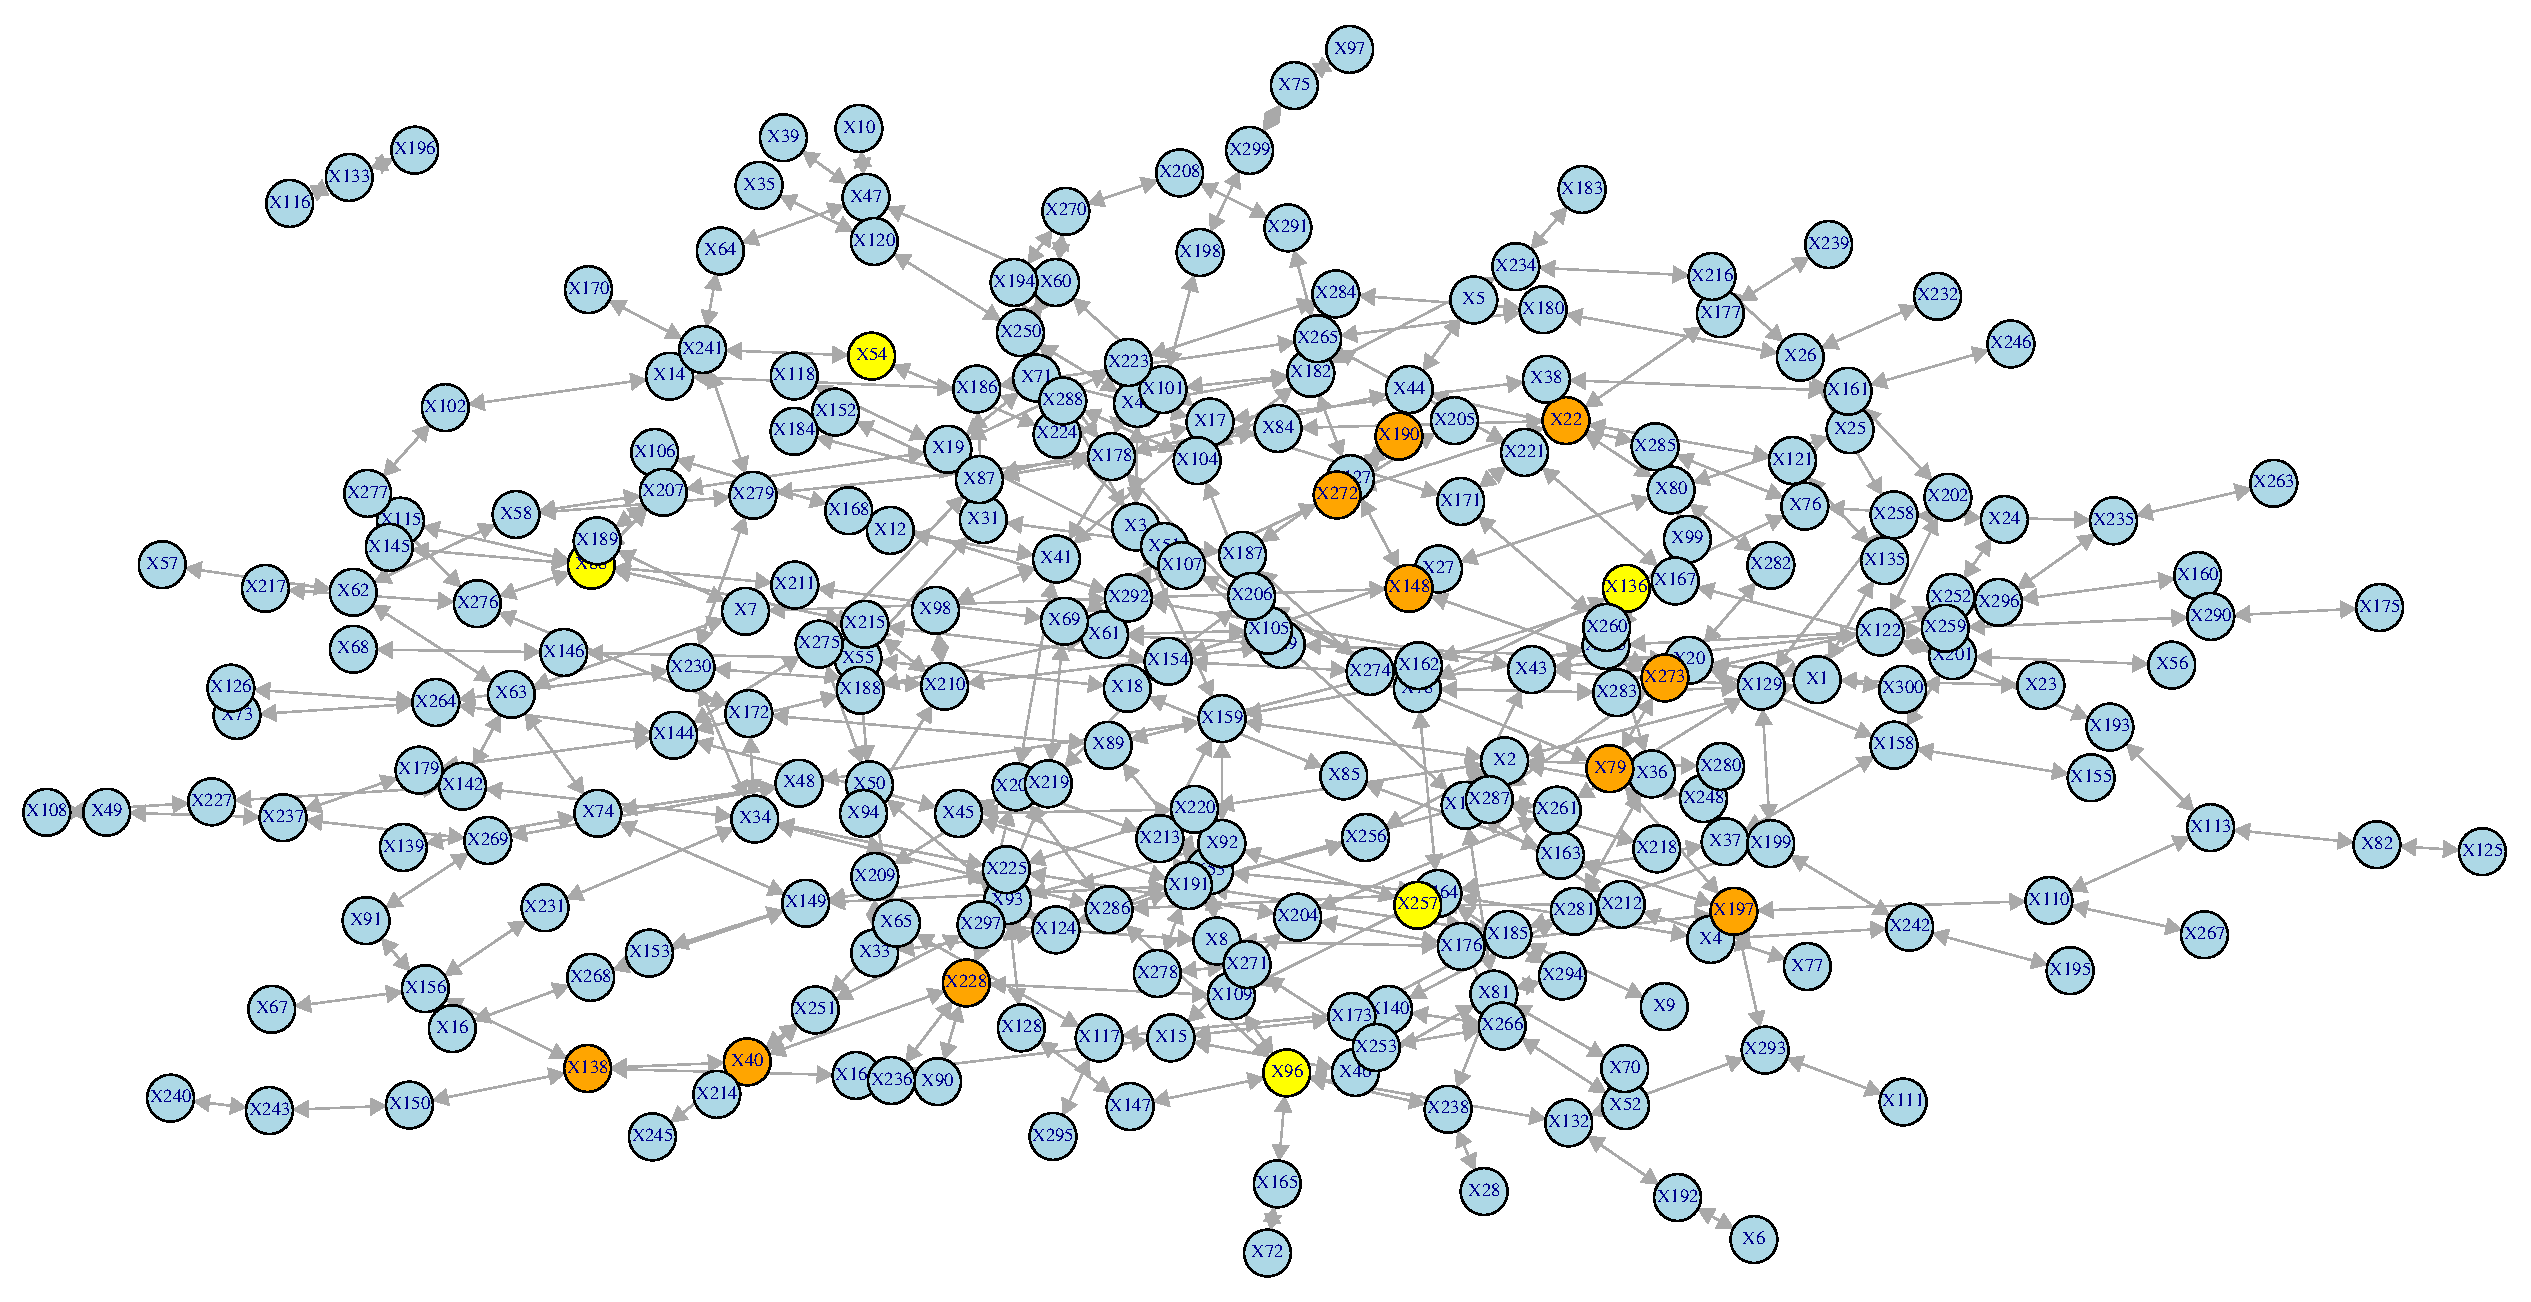
\includegraphics[width=0.8\textwidth]{synthesized-hard}
  \end{figure}
\end{frame}
\begin{frame}[plain]
  \frametitle{Synthesized data hard scenario}
  \begin{figure}
    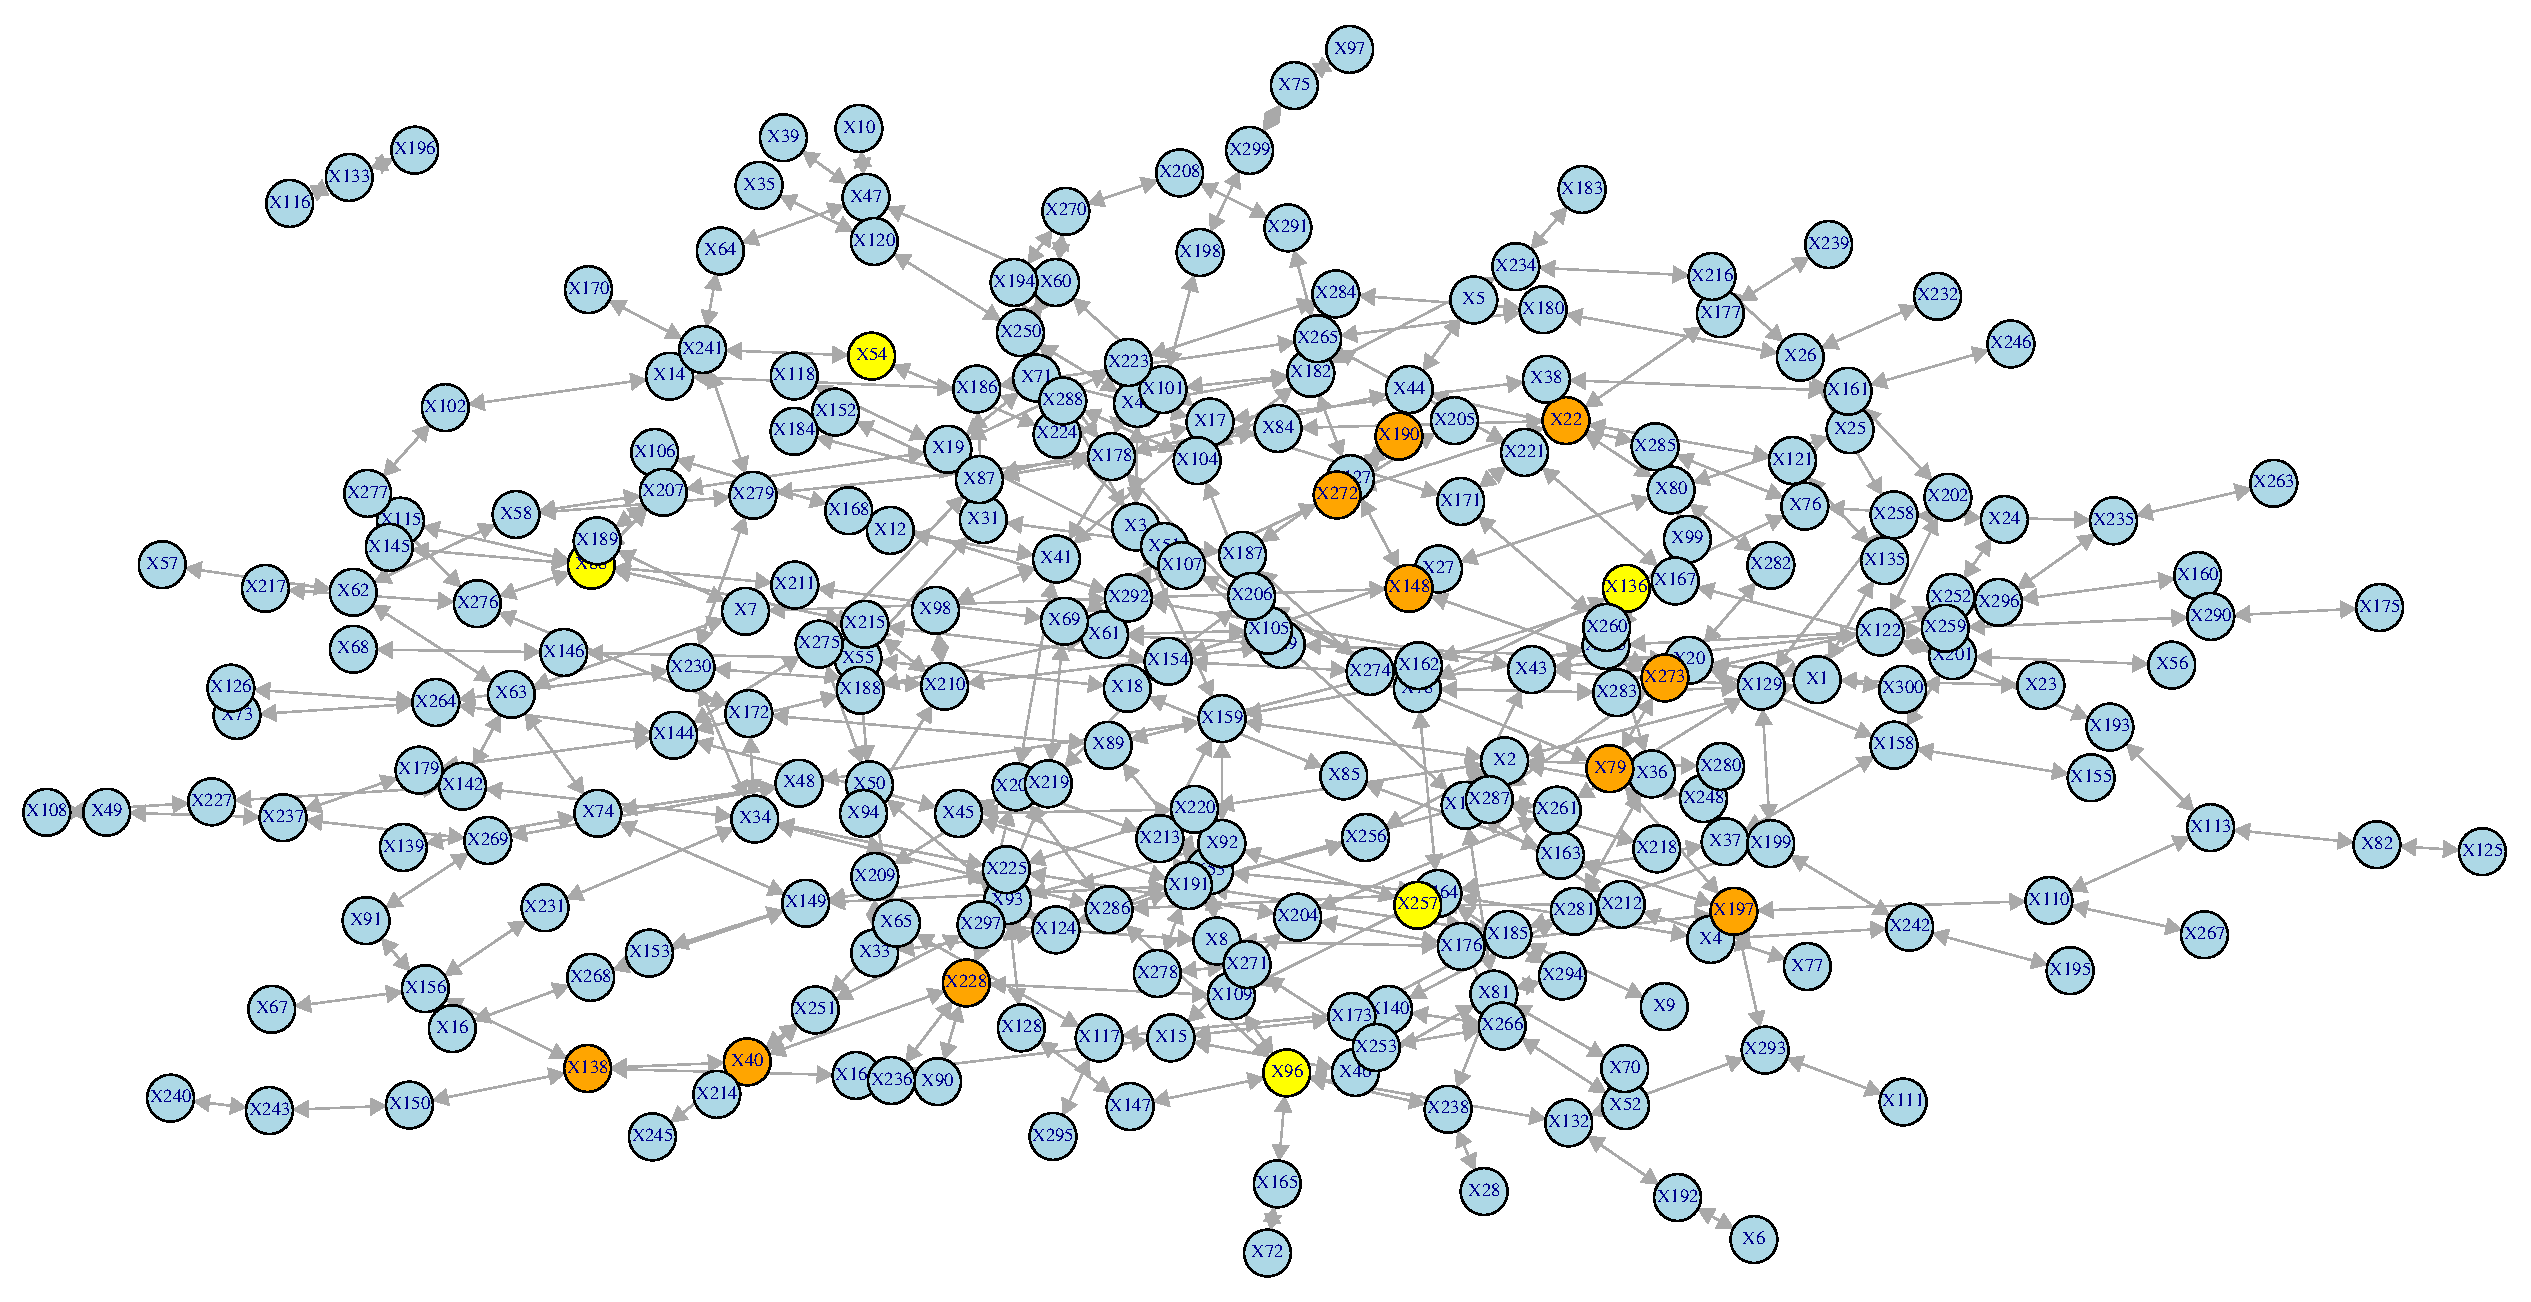
\includegraphics[width=0.8\textwidth]{synthesized-hard}
  \end{figure}
  \begin{textblock*}{\paperwidth}(0.01\textwidth,0.2\textheight)
    \raggedright 
    \tiny
    \begin{tabular}{| c c |}
      \hline
X42   &  X42  \\ \hline
X101   &  X101  \\ \hline
X106   &  X106  \\ \hline
X42   &  X182  \\ \hline
X101   &  X198  \\ \hline
X106   &  X168  \\ \hline
X12   &  X12  \\ \hline
X101   &  X182  \\ \hline
X198   &  X198  \\ \hline
X168   &  X168  \\ \hline
X42   &  X3  \\ \hline
X101   &  X41  \\ \hline
\boz X190   &  \boz X190  \\ \hline
X281   &  X281  \\ \hline
X98   &  X98  \\ \hline
\boz X190   &  X127  \\ \hline
X42   &  X250  \\ \hline
X182   &  X182  \\ \hline
X182   &  X127  \\ \hline
X147   &  X147  \\ \hline
X127   &  X127  \\ \hline
\boz X79   &  \boz X79  \\ \hline
X12   &  X41  \\ \hline
X205   &  X205  \\ \hline
X198   &  X299  \\ \hline
X127   &  X187  \\ \hline
X168   &  X292  \\ \hline
X127   &  \boz X148  \\ \hline
X187   &  X187  \\ \hline
X281   &  X36  \\ \hline
    \end{tabular}
    \hspace{.5em}
  \end{textblock*}
  \begin{textblock*}{\paperwidth}(1\textwidth,0.2\textheight)
    \raggedright 
    \tiny
    \begin{tabular}{| c c |}
      \hline
X97   &  X97  \\ \hline
X97   &  X75  \\ \hline
X75   &  X75  \\ \hline
X75   &  X299  \\ \hline
X299   &  X299  \\ \hline
X299   &  X198  \\ \hline
X106   &  X106  \\ \hline
X198   &  X198  \\ \hline
X106   &  X168  \\ \hline
X198   &  X101  \\ \hline
X205   &  X205  \\ \hline
X168   &  X168  \\ \hline
X205   &  \boz X272  \\ \hline
X101   &  X101  \\ \hline
\boz X190   &  \boz X190  \\ \hline
\boz X190   &  \boz X272  \\ \hline
X90   &  X90  \\ \hline
\boz X272   &  \boz X272  \\ \hline
X101   &  X182  \\ \hline
\boz X190   &  X127  \\ \hline
X236   &  X236  \\ \hline
\boz X272   &  X69  \\ \hline
X12   &  X12  \\ \hline
X69   &  X69  \\ \hline
X168   &  X292  \\ \hline
X69   &  X219  \\ \hline
X101   &  X41  \\ \hline
X90   &  \boz X228  \\ \hline
X236   &  \boz X228  \\ \hline
X219   &  X219  \\ \hline
    \end{tabular}
    \hspace{.5em}
  \end{textblock*}
\end{frame}

\begin{frame}
\frametitle{Results}
\begin{enumerate}
\item Extract pairs of genes with mutual absolute large $w$ 
\item Synthesized easy: all implanted pathways come on top of the list 
\item Synthesized hard: they are vanished \pause
\item Van't veer: 
  \begin{enumerate}
    \item Slightly better performance, although not necessarily as reported.
    \item You find even better genes in w/o network scenario.
    \item Well known genes are of very high degree in the network.
  \end{enumerate}
\end{enumerate}
\end{frame}

\section{Idea}
\begin{frame}
\frametitle{Idea}
\begin{enumerate}
\item Estimate density distribution of each gene for class A. \pause
\item For each sample:
  \begin{enumerate}
  \item Extract abnormal genes according to above estimated distributions.
  \item Extract the part of PPI network induced by extracted genes (almost)
  \end{enumerate}\pause
\item Use a graph kernel for labeled graphs to classify extracted graphs. \pause
\item Extract common sub-graphs from individual graphs that seem to be helping the classification.
\end{enumerate}
\end{frame}

\begin{frame}
  \frametitle{Why it doesn't work}
\end{frame}

\begin{frame}
  \frametitle{Weighted idea}
\end{frame}

\begin{frame}[plain]
\frametitle{Finished!}
  \begin{center}
    \Huge{Thank You!}
  \end{center}
\end{frame}

\end{document}
